% !TEX encoding = UTF-8 Unicode

%
% Exemple de rapport
% par Pierre Tremblay, Universite Laval
% modifié par Christian Gagne, Universite Laval
% modifié par Francis Valois, Université Laval
% 31/01/2011 - version 1.4
%

%
% Modele d'organisation d'un projet LaTeX 
% rapport/      dossier racine et fichier principal
% rapport/fig   fichiers des figures
% rapport/tex   autres fichiers .tex
%

% ** Preambule **
%
% Ajouter les options au besoin :
%    - "ULlof" pour inclure la liste des figures, requis si "\begin{figure}" utilise
%    - "ULlot" pour inclure la liste des tableaux, requis si "\begin{table}" utilise
%
\documentclass[12pt,ULlof,ULlot]{ULrapport}

% Chargement des packages supplementaires (si absent de la classe)
\usepackage[utf8]{inputenc}
\usepackage[T1]{fontenc}
\usepackage[autolanguage]{numprint}
\usepackage{icomma}
\usepackage{subfigure}
\usepackage{graphicx}
\usepackage[absolute]{textpos}
\usepackage[final]{pdfpages}
\usepackage{listings} % For source code
\usepackage{color}
\usepackage{pdflscape}
\usepackage{multirow}
\usepackage{array}
% settings pour le listing de code
\lstset{
	tabsize=4,
	language=matlab,
        basicstyle=\scriptsize,
        %upquote=true,
        aboveskip={1.5\baselineskip},
        columns=fixed,
        showstringspaces=false,
        extendedchars=true,
        breaklines=true,
        prebreak = \raisebox{0ex}[0ex][0ex]{\ensuremath{\hookleftarrow}},
	frame=single,
        showtabs=false,
        showspaces=false,
        showstringspaces=false,
        identifierstyle=\ttfamily,
        keywordstyle=\color[rgb]{0,0,1},
        commentstyle=\color[rgb]{0.133,0.545,0.133},
        stringstyle=\color[rgb]{0.627,0.126,0.941},
	language=Java
}
\newcommand{\HRule}{\rule{\linewidth}{0.2mm}}
%\usepackage[hmargin=3cm,vmargin=3.5cm]{geometry}
\definecolor{mygrey}{gray}{.96} % Light Grey
\lstset{ 
	language=vhdl,              % choose the language of the code
%("language=Verilog" is popular as well)
	tabsize=4,			% sets the size of the tabs in spaces (1
%Tab is replaced with 3 spaces)
	basicstyle=\scriptsize,               % the size of the fonts that are
%used for the code
	numbers=left,                   % where to put the line-numbers
	numberstyle=\tiny,              % the size of the fonts that are used
%for the line-numbers
	stepnumber=1,                   % the step between two line-numbers. If
%it's 1 each line will be numbered
	numbersep=5pt,                  % how far the line-numbers are from the
%code
	backgroundcolor=\color{mygrey}, % choose the background color. You must add \usepackage{color}
	showspaces=false,              % show spaces adding particular underscores
	showstringspaces=false,        % underline spaces within strings
	%showtabs=false,                % show tabs within strings adding particular underscores
	frame=single,	                 % adds a frame around the code
	tabsize=3,	                    % sets default tabsize to 2 spaces
	captionpos=b,                   % sets the caption-position to bottom
	breaklines=true,                % sets automatic line breaking
	breakatwhitespace=false,        % sets if automatic breaks should only happen at whitespace
	%escapeinside={\%*}{*)},        % if you want to add a comment within your code
	%commentstyle=\color{RedBrick}   % sets the comment style
}

\def\dbar{{\mathchar'26\mkern-12mu d}} 
%\usepackage[options]{nom_du_package}

% Definition d'une commande pour presenter des cellules multilignes dans un tableau
\newcommand{\cellulemultiligne}[1]{\begin{tabular}{@{}c@{}}#1\end{tabular}}


% Definition de colonnes en mode paragraphe avec alignement ajustable
% Cette definition requiert le chargement du package "array"
%    - alignement horizontal, parametre #1 : - \raggedright (aligne a gauche)
%                                            - \centering (centre)
%                                            - \raggedleft (aligne a droite)
%    - alignement vertical, parametre #2 : - p (aligne en haut)
%                                          - m (centre)
%                                          - b (aligne en bas)
%    - largeur, parametre #3 : longueur
\newcolumntype{Z}[3]{>{#1\hspace{0pt}\arraybackslash}#2{#3}}

% Definitions des parametres de la page titre
\TitreProjet{Livrable 2 - Robot Kinocto}                         % Titre du projet
\TitreRapport{Design III}       % Titre du rapport
\Destinataire{M. Dominique Grenier, M. Luc Lamontagne et M. Abdelhakim Bendada}         % Nom(s) du destinataire
\TableauMembres{%                                     % Tableau des membres de l'equipe
   910\,058\,073  & Émile Arsenault \\\hline 
   908\,190\,985  & Philippe Bourdages \\\hline
   910\,098\,468  & Pierre-Luc Buhler \\\hline    
   998\,107\,355  & Diane Fournier \\\hline
   908\,159\,170  & Imane Mouhtij \\\hline
   908\,318\,388  & Olivier Sylvain \\\hline
   910\,055\,897  & Daniel Thibodeau \\\hline
   910\,097\,879  & Francis Valois \\\hline
}
\DateRemise{7 mars 2013}                           % Date de remis


% Corps du document

\begin{document}

%   Chapitres
%!TEX root = ../rapport.tex
%!TEX encoding = UTF-8 Unicode

% Chapitres "Introduction"

% modifié par Francis Valois, Université Laval
% 31/01/2011 - version 1.0 - Création du document

\chapter{Introduction}
\label{s:introduction}

%!TEX root = ../rapport.tex
%!TEX encoding = UTF-8 Unicode

% Chapitres "Introduction"

% modifié par Francis Valois, Université Laval
% 31/01/2011 - version 1.0 - Création du document

\chapter{Diagramme des fonctionnalités}
\label{s:diagfonct}
%!TEX root = ../rapport.tex
%!TEX encoding = UTF-8 Unicode

% Chapitres "Introduction"

% modifié par Francis Valois, Université Laval
% 31/01/2011 - version 1.0 - Création du document

\chapter{Diagramme physique}
\label{s:physique}

Le diagramme physique est présenté à la figure \ref{fig:diag_physique}. Il est séparé en trois sous-composantes qui sont respectivement : la kinect, la station de base et le robot. Chaque flèche correspond à une interaction entre composantes et peut être soit unidirectionnelle ou bidirectionnelle. De plus, chacun des protocoles ou types d'information sont écrits sur l'interaction pour aider à la compréhension du flux de données dans le projet. Finalement, chacune des boîtes à l'extérieur du rectangle principal correspond à des entrées-sorties nécessaires pour la réussite du projet. Pour permettre une meilleure compréhension du diagramme et éviter une surcharge de celui-ci, les fonctionnalités effectuées par chacune des composantes sont énumérées dans les tableaux \ref{tab:diag_physique1}, \ref{tab:diag_physique2} et \ref{tab:diag_physique3}.


\begin{table}[!ht]
	\caption{Matrice de liaisons entre les composantes physiques et les fonctionnalités effectuées : Kinect} 
	\label{tab:diag_physique1}
	\tabcolsep=0.11cm
	\centering
	\begin{tabular}{|Z{\raggedright}{m}{6.5 cm}|Z{\raggedright}{m}{6.5 cm}|}
	\hline
	Composantes & Fonctionnalités \\ \hline\hline
	\multirow{2}{6.5cm}{Caméra RGB}	& Détecter les obstacles \\ \cline{2-2}
			   						& Localiser le robot \\ \hline
	\multirow{2}{6.5cm}{Caméra infra-rouge} & Détecter les obstacles \\ \cline{2-2}
											& Localiser le robot \\ \hline
	Ordinateur embarqué & Transfert des images de la Kinect vers le Mac mini \\ \hline
	\end{tabular}
\end{table}

\begin{table}[!ht]
	\caption{Matrice de liaisons entre les composantes physiques et les fonctionnalités effectuées : Station de base} 
	\label{tab:diag_physique2}
	\tabcolsep=0.11cm
	\centering
	\begin{tabular}{|Z{\raggedright}{m}{6.5 cm}|Z{\raggedright}{m}{6.5 cm}|}
	\hline
	Composantes & Fonctionnalités \\ \hline\hline
	 & Détecter les obstacles \\ \cline{2-2}
	\multirow{3}{6.5cm}{Ordinateur}& Communiquer entre le robot et la station de base \\ \cline{2-2}
	& Localiser le robot\\ \cline{2-2}
	& Transfert des images de la Kinect vers le Mac mini \\ \hline
	\multirow{7}{6.5cm}{Interface}& Afficher la trajectoire optimale \\ \cline{2-2}
	& Afficher la position du robot\\ \cline{2-2}
	& Afficher le temps d'exécution\\ \cline{2-2}
	& Afficher message d'initiation de la tâche \\ \cline{2-2}
	& Afficher message de fin \\ \cline{2-2}
	& Afficher le cube résolu \\ \hline
	\end{tabular}
\end{table}


\begin{table}[!ht]
	\caption{Matrice de liaisons entre les composantes physiques et les fonctionnalités effectuées : Robot} 
	\label{tab:diag_physique3}
	\tabcolsep=0.11cm
	\centering
	\begin{tabular}{|Z{\raggedright}{m}{6.5 cm}|Z{\raggedright}{m}{8 cm}|}
	\hline
	Composantes & Fonctionnalités \\ \hline\hline
	\multirow{11}{6.5cm}{Mac mini} 	& Détecter les obstacles \\ \cline{2-2}
									& Choisir le cube selon le signal d'antenne \\ \cline{2-2}
									& Calcul de la trajectoire optimale\\ \cline{2-2}
									& Transmettre la trajectoire optimale\\ \cline{2-2}
									& Contrôler le robot pour le dessin \\ \cline{2-2}
									& Commander le préhenseur\\ \cline{2-2}
									& Contrôler la position de la caméra\\ \cline{2-2}
									& Résoudre le cube \\ \cline{2-2}
									& Commander les moteurs \\ \cline{2-2}
									& Allumer la DEL lorsque la tâche est complétée \\ \hline
	Écran LCD & Afficher sur le LCD \\ \hline
	\multirow{6}{6.5cm}{Micro-contrôleur}	& Décodage du signal d'antenne \\ \cline{2-2}
											& Contrôler le robot pour le dessin \\ \cline{2-2}
											& Commander le préhenseur\\ \cline{2-2}
											& Commander les moteurs \\ \cline{2-2}
											& Allumer la DEL lorsque la tâche est complétée \\ \hline
	\multirow{2}{6.5cm}{Batterie} 	& Utiliser une pile rechargeable \\ \cline{2-2}
									& Alimenter les moteurs \\ \hline
	
	Alimentation hacheur 5V & Alimenter les différents périphériques \\ \hline
	Alimentation survolteur 24V & Alimenter l'ordinateur et les différents périphériques\\ \hline
	Pont en H & Commander les moteurs \\ \hline
	Moteurs de déplacement & Se déplacer sans toucher aux obstacles \\ \hline
	Circuit d'antenne & Réception du signal d'antenne \\ \hline
	Antenne & Réception du signal d'antenne \\ \hline
	Moteurs de la caméra & Contrôler la position de la caméra \\ \hline
	Circuit de contrôle des moteur de la caméra & Contrôler la position de la caméra \\ \hline
	Circuit de contrôle de la LED & Allumer la DEL lorsque la tâche est complétée \\ \hline
	Circuit de contrôle du préhenseur & Commander le préhenseur \\ \hline
	\multirow{4}{6.5cm}{Caméra} 	& Détecter les obstacles \\ \cline{2-2}
								& Transmettre les images de la caméra vers le Mac mini \\ \cline{2-2}
								& Lire le cube \\ \hline



	\end{tabular}
\end{table}


\begin{figure}[htbp]
\centering
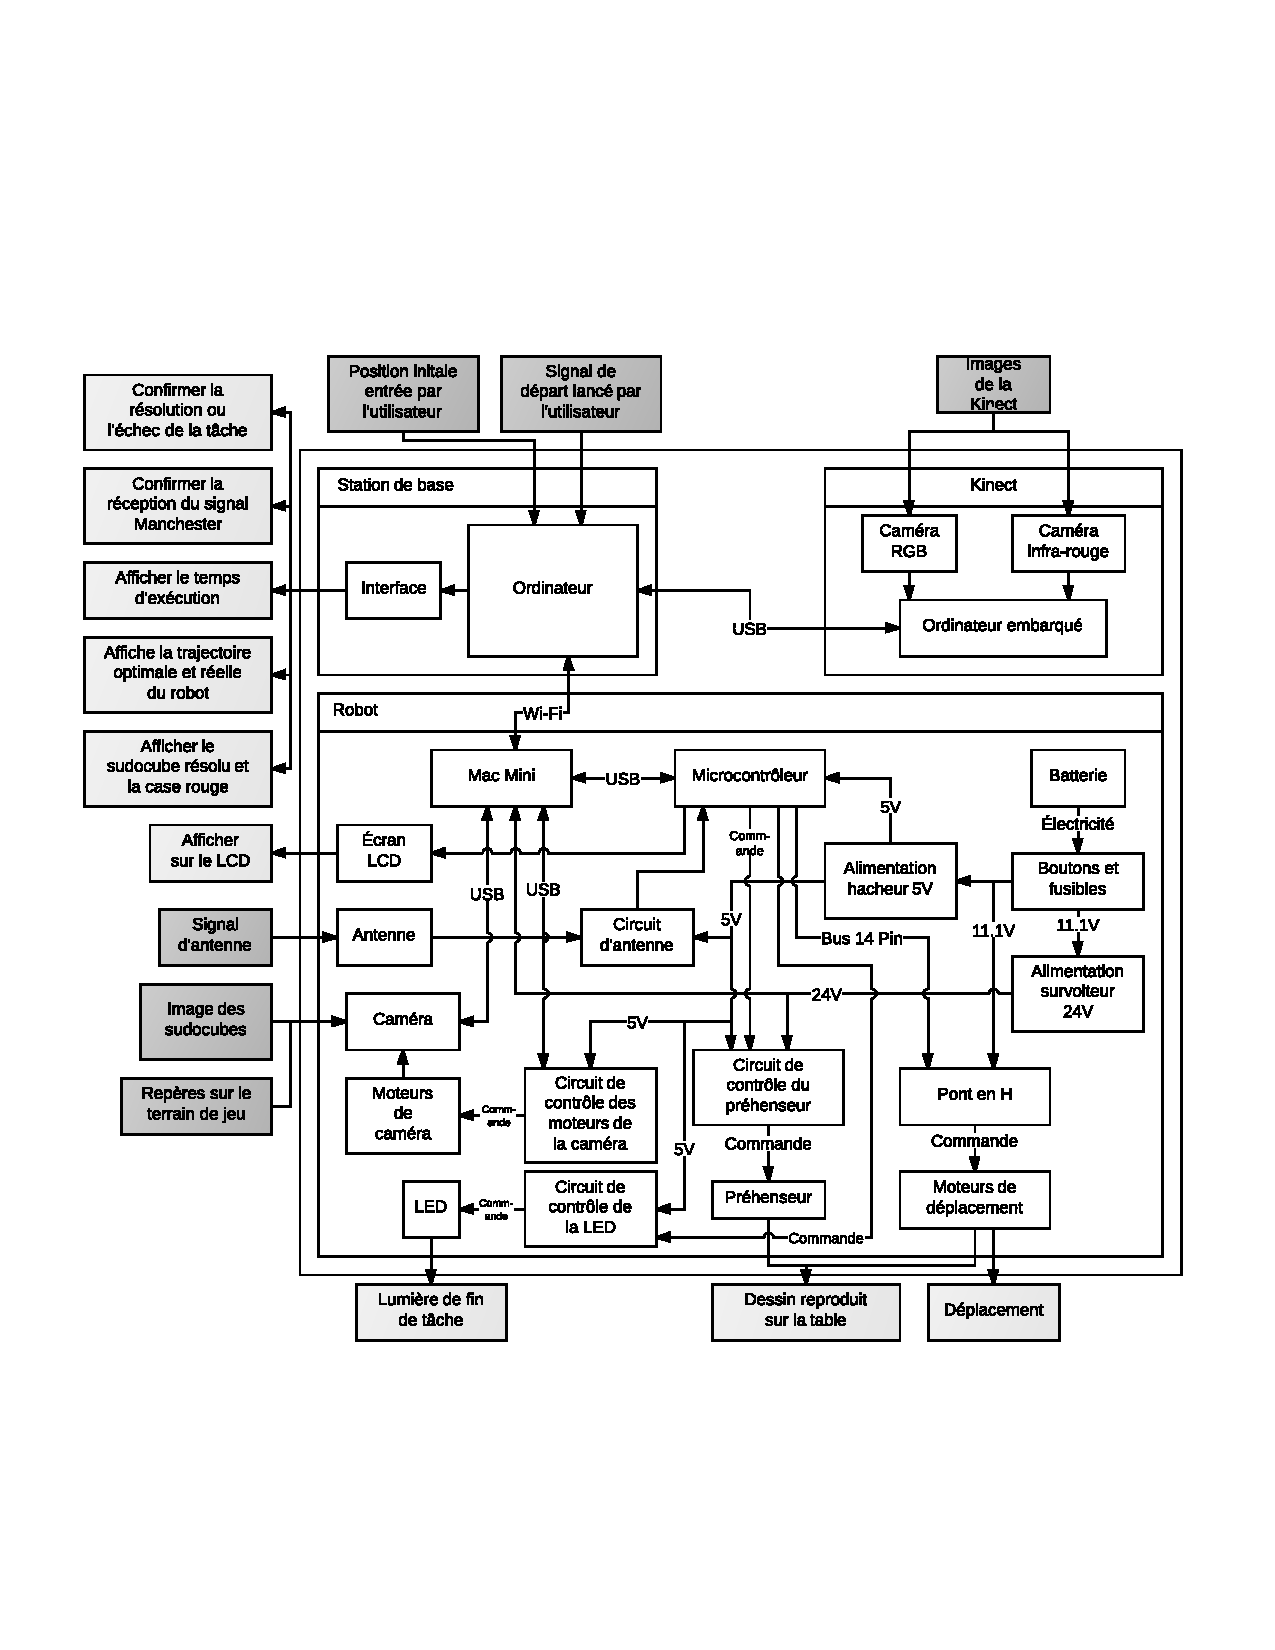
\includegraphics[scale=0.9]{fig/diag_physique.pdf}
\caption{Diagramme physique de l'implantation du robot Kinocto}
\label{fig:diag_physique}
\end{figure}


%!TEX root = ../rapport.tex
%!TEX encoding = UTF-8 Unicode

% Chapitres "Introduction"

% modifié par Francis Valois, Université Laval
% 31/01/2011 - version 1.0 - Création du document
\chapter{Diagrammes de classes}
	\label{s:classes}
	\addtolength{\evensidemargin}{-1in}	

\begin{figure}[htbp]
\centering
\label{fig:DiagrammeClasse}
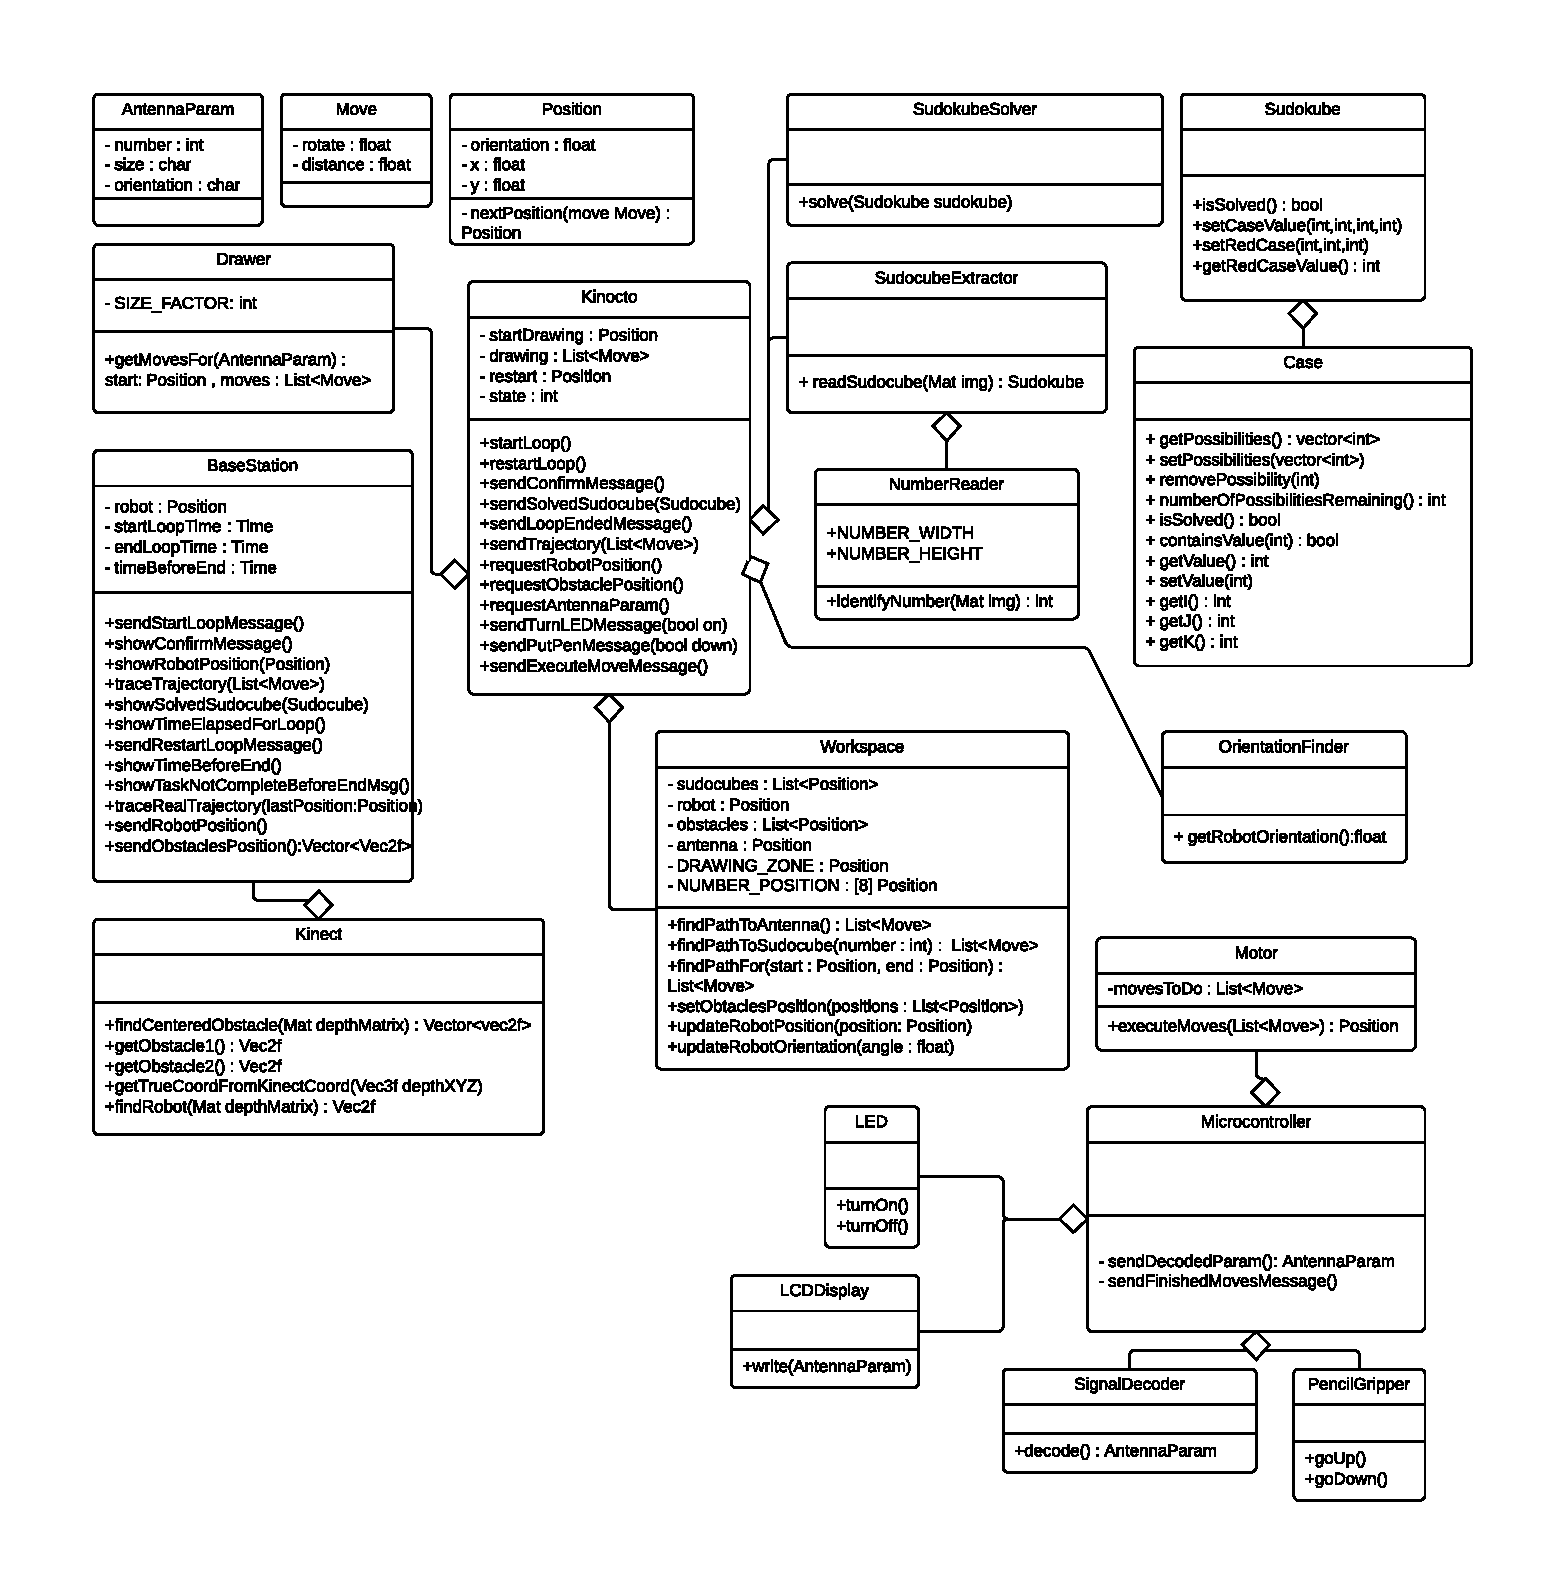
\includegraphics[scale=0.60]{fig/class_diagram.pdf}
\caption{Figure présentant le diagramme de classes du projet}
\end{figure}

%!TEX root = ../rapport.tex
%!TEX encoding = UTF-8 Unicode

% Chapitres "Introduction"

% modifié par Francis Valois, Université Laval
% 31/01/2011 - version 1.0 - Création du document

\chapter{Diagrammes de séquences}
\label{s:sequences}

%!TEX root = ../rapport.tex
%!TEX encoding = UTF-8 Unicode

% Chapitres "Introduction"

% modifié par Francis Valois, Université Laval
% 31/01/2011 - version 1.0 - Création du document
\chapter{Registre de risques}
\begin{landscape}
\begin{table}[htbp]
	\small
 	 \centering
  	\caption{Registre de risques partie 1}
  	\scalebox{0.8}{
	\tabcolsep=0.11cm
    \begin{tabular}{|Z{\centering}{m}{1.5cm}||Z{\raggedright}{p}{3cm}|Z{\raggedright}{m}{1.5cm}|Z{\raggedright}{p}{5cm}|Z{\raggedright}{p}{4cm}|Z{\centering}{m}{1.5cm}|Z{\centering}{m}{1.5cm}|Z{\raggedright}{p}{4cm}|Z{\raggedright}{p}{3cm}|}\hline
    \textbf{Risque} &\textbf{Type de risque} &\textbf{Niveau de priorité (1- faible, 5-élevé)} & \textbf{Conséquences de l'occurrence du risque} & \textbf{Coût en performance associé au risque} & \textbf{Prob. d'occurrence (\%)} & \textbf{Coût estimé du risque (\$)}& \textbf{Plan de réduction du risque} & \textbf{Responsable du risque} \\\hline\hline
    1 & Bris  de la batterie Li-Po suite à une mauvaise utilisation & 5 & Plus d'autonomie énergétique pour le robot, opération impossible & L'ensemble du système sera inopérable &5 & 60 & Formation des utilisateurs à l'endroit de l'utilisation. Apposition d'un capteur de tension. Dispositifs de protection (fusibles) & É. Arsenault \\\hline
    2 & Bris  d'un ou des système d'alimentation & 5 & Les systèmes auxiliaires, le Mac mini ou les moteurs ne seront pas alimentés. Le système ne sera pas fonctionnel & Une partie ou l'ensemble du système sera inopérable & 5 & 25 & Utilisateur de connecteurs protégés (d'un seul sens possible). Dispositifs de protection (fusibles), surdimensionnement des composantes d'alimentation. Achat de pièces de rechange. & D. Thibodeau \\\hline
    3 & Bris  du crayon lors du dessin & 4 & Le dessin ne pourra être complété & La portion dessin sera partiellement complète & 20 & 2 & Tests rigoureux et optimisation du choix de crayon avant la compétition & É. Arsenault \\\hline
    4 & Bris du système de préhension & 5 & Le dessin ne pourra être complété et selon le moment du bris, la trajectoire du robot peut être affectée & La portion dessin sera partiellement complète et la trajectoire sera déviée & 5 & 10 & Tests rigoureux et essais multiples pour vérifier la stabilité en température lors du fonctionnement  & É. Arsenault \\\hline
    5 & Problèmes de réception ou de décodage du signal d'antenne & 4 & Si la réception est erronée, le robot peut exécuter sa séquence, mais l'exécution ne sera pas conforme au message. Si la réception est impossible, le système ne s'amorcera pas. & Accomplissement de la mauvaise tâche ou système non fonctionnel & 5 & 15 & Tests répétés pour un taux de succès de 100\% lors de la réception et du décodage avec ajout de sources de bruit externes. & D.Fournier \\\hline
   
    \end{tabular}}%
  \label{tab:rr1}%
\end{table}%
\end{landscape}
\begin{landscape}
\begin{table}[htbp]
	\small
 	 \centering
  	\caption{Registre de risques partie 2}
  	\scalebox{0.8}{
	\tabcolsep=0.11cm
    \begin{tabular}{|c||p{3cm}|>{\centering\arraybackslash}m{1.5cm}|p{4.8cm}|p{4.6cm}|>{\centering\arraybackslash}m{1.5cm}|>{\centering\arraybackslash}m{1.5cm}|p{4cm}|p{3cm}|}\hline
    \textbf{Risque} &\textbf{Type de risque} &\textbf{Niveau de priorité (1- faible, 5-élevé)} & \textbf{Conséquences de l'occurrence du risque} & \textbf{Coût en performance associé au risque} & \textbf{Prob. d'occurrence (\%)} & \textbf{Coût estimé du risque (\$)}& \textbf{Plan de réduction du risque} & \textbf{Responsable du risque} \\\hline\hline
    
    6 & Bris du pont en H & 5 & Les moteurs ne pourront être commandés correctement & Le robot ne peut pas se déplacer, le système n'est pas fonctionnel & 5 & 130 & Utilisation d'un régulateur de type PID afin d'éviter les appels brusques de courants, positionnement du pont de manière à limiter son exposition aux accrochages & F. Valois \\\hline
    
    7 & Bris d'une portion ou de la totalité du microcontrôleur & 4 & Le bris d'une portion du microcontrôleur empêche l'exécution de la tâche dans son ensemble et peut occasionner des bris dans les systèmes reliés & Un robot qui ne peut pas se déplacer correctement, qui n'allume pas la DEL ou qui n'active pas le préhenseur & 5 & 100 & Isolation des entrées et sorties avec des dispositifs de protection (diode), limiteur de courant & D. Fournier \\\hline
    
    8 & Bris du Mac mini & 5 & L'ensemble des auxiliaires ne fonctionnera pas correctement. Le système sera non fonctionnel & Robot incapable de se déplacer selon la trajectoire prévue et d'effectuer la tâche & 5 &  600  & Apposition de protections électriques (fusibles et interrupteurs) sur l'étage d'alimentation du Mac mini. Fixation robuste du Mac mini sur le robot. Protection du port USB du Mac mini en n'utilisant pas le fil d'alimentation. & F. Valois \\\hline
    
    9 & Caméra web désaxée & 3 & Les prises de données du sudo cube seront affectées & L'acquisition des données du sudo cube pourrait être non fonctionnelle et causer une erreur dans la résolution du cube & 10 &       & Tests rigoureux d'asservissement de la caméra et de retour à l'axe désiré suivant une modification externe. & P. Buhler \\\hline
    
    10 & Bris de la caméra web & 4 & Le bris de la caméra empêche la vision des cubes & Si la caméra ne peut voir le sudo cube, on ne peut trouver le chiffre dans la case rouge et effectuer le bon dessin & 5 & 80 & Storage adéquat de la caméra, protection d'alimentation (fusible), limiter les chocs contre les obstacles & D. Thibodeau \\\hline


    
\end{tabular}}%
  \label{tab:rr2}%
\end{table}%
\end{landscape}
\begin{landscape}
\begin{table}[htbp]
	\small
 	 \centering
  	\caption{Registre de risques partie 3}
  	\scalebox{0.8}{
	\tabcolsep=0.11cm
    \begin{tabular}{|c||p{3cm}|>{\centering\arraybackslash}m{1.5cm}|p{4cm}|p{4cm}|>{\centering\arraybackslash}m{1.5cm}|>{\centering\arraybackslash}m{1.5cm}|p{5cm}|p{3cm}|}\hline
    \textbf{Risque} &\textbf{Type de risque} &\textbf{Niveau de priorité (1- faible, 5-élevé)} & \textbf{Conséquences de l'occurrence du risque} & \textbf{Coût en performance associé au risque} & \textbf{Prob. d'occurrence (\%)} & \textbf{Coût estimé du risque (\$)}& \textbf{Plan de réduction du risque} & \textbf{Responsable du risque} \\\hline\hline

 	11 & Problème de communication entre le Mac mini et la station de base & 5 & Les informations requises ne pourront être transmises correctement, on perd l'information sur le comportement du robot ainsi que sa position. Le robot ne pourra pas se localiser initialement et en temps réel. & Le robot de remplira pas les exigences d'affichage sur la station de base, le robot ne recevra aucune position de la Kinect  & 5 &       & Tests répétés pour un taux de succès de près de 100\% lors de la transmission et de la réception de l'information en temps réel entre le Mac mini et la station de base & P. Bourdages \\\hline
 	12 & Bris du système d'exploitation du Mac mini & 4 & La portion logicielle du robot et le traitement seront absents. Le système ne sera pas fonctionnel & Robot incapable d'accomplir un traitement de tâches & 30 &       &Clonage d'une version fonctionnelle et stable du système d'exploitation & P. Buhler \\\hline
 	13 & Problème de communication entre le Mac mini et le microcontrôleur & 5 & L'ensemble des auxiliaires ne fonctionnera pas correctement. Le système sera non fonctionnel & Robot incapable de se déplacer selon la trajectoire prévue et d'effectuer la tâche & 5 &       & Tests répétés pour un taux de succès de près de 100\% lors de la transmission et de la réception de l'information entre le Mac mini et le microcontrôleur & D. Fournier \\\hline
 	14 & Contact avec un ou des obstacles & 3 & Bris du système et déviation de trajectoire possible & Un robot qui entre en contact avec les obstacles ne remplit pas les exigences du projet & 20 &       & Tests rigoureux sur les déplacements et marge de sécurité importante pour le contournement. & O. Sylvain \\\hline
    
    \end{tabular}}%
  \label{tab:rr3}%
\end{table}%
\end{landscape}

\begin{landscape}
\begin{table}[htbp]
	\small
 	 \centering
  	\caption{Registre de risques partie 4}
  	\scalebox{0.8}{
	\tabcolsep=0.11cm
    \begin{tabular}{|c||p{3cm}|>{\centering\arraybackslash}m{1.5cm}|p{4cm}|p{5cm}|>{\centering\arraybackslash}m{1.5cm}|>{\centering\arraybackslash}m{1.5cm}|p{4cm}|p{3cm}|}\hline
    \textbf{Risque} &\textbf{Type de risque} &\textbf{Niveau de priorité (1- faible, 5-élevé)} & \textbf{Conséquences de l'occurrence du risque} & \textbf{Coût en performance associé au risque} & \textbf{Prob. d'occurrence (\%)} & \textbf{Coût estimé du risque (\$)}& \textbf{Plan de réduction du risque} & \textbf{Responsable du risque} \\\hline\hline
	15 & Problème d'identification du robot et de l'environnement (vision) par la Kinect & 5 & Correction de la trajectoire erronée, risque de rencontrer les obstacles, mauvaise trajectoire calculée & La trajectoire réelle ne sera pas optimale et le robot risque de rencontrer des obstacles & 10 &  & Tests rigoureux et taux de succès de l'identification proche de 100\% & I. Mouhtij \\\hline
 	16 & Perturbations de l'environnement du robot (irrégularités sur la table ou dans l'éclairage) &2 & La trajectoire du robot pourrait être 			déviée si la vision est entachée par une mauvaise luminosité ou une irrégularité dans la table & La trajectoire parcourue par le robot ne 			sera pas idéale& 10 &  & Tests rigoureux des algorithmes de vision et d'asservissement, essais avec ajout d'irrégularités & D. Thibodeau 			\\\hline
 	    
    17 & Départ de l'un des membres de l'équipe & 3 & La quantité de tâches des membres restants de l'équipe devra être augmentée. & Des détails et des ajustements de pointes nécessitant plus de temps ne seront pas réalisés& 5 &       & S'assurer d'une bonne communication dans l'équipe et d'un bon transfert de conaissances& D. Thibodeau\\\hline
    
 
   \end{tabular}}%
  \label{tab:rr4}%
\end{table}%
\end{landscape}


%!TEX root = ../rapport.tex
%!TEX encoding = UTF-8 Unicode

% Chapitres "Introduction"

% modifié par Francis Valois, Université Laval
% 31/01/2011 - version 1.0 - Création du document

\chapter{Plan de tests}
\label{s:plantest}
\begin{landscape}
\begin{table}[htbp]
	\small
 	 \centering
  	\caption{Plan de tests côté matériel (partie 1)}
  	\scalebox{0.8}{
	\tabcolsep=0.11cm
    \begin{tabular}{|Z{\centering}{m}{4cm}||Z{\centering}{m}{5cm}|Z{\centering}{m}{5cm}|Z{\centering}{m}{3cm}|Z{\centering}{m}{4cm}|Z{\centering}{m}{5cm}|}\hline
    \textbf{Fonctionnalité}& \textbf{Sous-fonctionnalité} & \textbf{Exigence}& \textbf{Méthode de vérification}& \textbf{Équipement requis}& \textbf{Méthode d'analyse}\\ \hline\hline
    
    \multirow{4}{4cm}{\centering Traitement numérique} & \multirow{4}{5cm}{\centering Contrôler le robot pour le dessin}& \multirow{4}{5cm}{\centering Précision de $\pm$1cm de la ligne centrale}&\multirow{4}{3cm}{\centering Tests pratiques}& \multirow{1}{4cm}{\centering Robot fonctionnel}& \multirow{4}{5cm}{\centering Effectuer l'ensemble des dessins 3 fois et mesurer l'écart maximal}\\\cline{5-5}
    & & &  																											& Ruban à mesurer  & \\\cline{5-5}
    & & &  																											& Gabarits des dessins& \\\cline{5-5}
    & & &  																											& Crayon              &\\\hline
    \multirow{4}{4cm}{\centering Déplacement} & \multirow{4}{5cm}{\centering Se déplacer sans toucher aux obstacles}& \multirow{4}{5cm}{\centering Distance minimale de 1cm par rapport à l'axe de la trajectoire et vitesse supérieure à 3cm/s}&\multirow{4}{3cm}{\centering Tests pratiques}& \multirow{1}{4cm}{\centering Robot fonctionnel}& \multirow{4}{5cm}{\centering Vérifier la déviation maximale ainsi que la vitesse moyenne pour une dizaine de trajectoires différentes}\\\cline{5-5}
    & & &  																											& Ruban à mesurer  & \\\cline{5-5}
    & & &  																											& Crayon& \\\cline{5-5}
    & & & 																											& Rapporteur d'angle&\\\hline
    
     \multirow{5}{4cm}{\centering Alimentation} & \multirow{5}{5cm}{\centering Alimenter le mac-mini et le préhenseur à une tension de 24 volts}& \multirow{5}{5cm}{\centering Fournir une tension de 24 volts CC avec des oscillations maximum de 1 volt}&\multirow{5}{3cm}{\centering Tests de mesure}& \multirow{1}{4cm}{\centering Mac mini}& \multirow{5}{5cm}{\centering Vérifier la tension moyenne à la sortie de l'alimentation et l'amplitude des oscillations qui y sont superposées sur l'oscilloscope}\\\cline{5-5}
    & & &  																											& \multirow{2}{4cm}{\centering Oscilloscope} & \\
    & & &  																											& & \\\cline{5-5}	
    & & &  																											& \multirow{2}{4cm}{\centering Sondes de mesure} & \\
    & & &  																											& & \\\hline											
    \multirow{5}{4cm}{\centering Alimentation} & \multirow{5}{5cm}{\centering Alimenter le micro-contrôleur et les différents circuits à une tension de 5 volts}& \multirow{5}{5cm}{\centering Fournir une tension de 5 volts CC avec des oscillations maximum de 0.2 volt}&\multirow{5}{3cm}{\centering Tests de mesure}& \multirow{1}{4cm}{\centering Robot fonctionnel}& \multirow{5}{5cm}{\centering Vérifier la tension moyenne à la sortie de l'alimentation et l'amplitude des oscillations qui y sont superposées sur l'oscilloscope}\\\cline{5-5}
    & & &  																											& \multirow{2}{4cm}{\centering Oscilloscope} & \\
    & & &  																											& & \\\cline{5-5}	
    & & &  																											& \multirow{2}{4cm}{\centering Sondes de mesure} & \\
    & & &  																											& & \\\hline     
     
     \multirow{4}{4cm}{\centering Récepteur manchester} & \multirow{4}{5cm}{\centering Recevoir le signal manchester et le rendre utilisable par le micro-contrôleur}& \multirow{4}{5cm}{\centering Fournir un signal carré 0-5 volts à l'image du signal reçu}&\multirow{4}{3cm}{\centering Tests de mesure}& \multirow{1}{4cm}{\centering Robot fonctionnel}& \multirow{3}{5cm}{\centering Vérifier la présence du signal carré en sortie du module de réception lorsque le robot est à proximité de l'antenne }\\\cline{5-5}
    & & &  																											& Oscilloscope & \\\cline{5-5}
     & & &  																											& Antenne fonctionnelle & \\\cline{5-5}
    & & &  																											& Sondes de mesure & \\\hline
     \multirow{5}{4cm}{\centering Préhenseur} & \multirow{5}{5cm}{\centering Monter et descendre le crayon pour passer en mode écriture ou arrêt d'écriture}& \multirow{5}{5cm}{\centering Descendre le crayon lorsqu'une commande 5V est apliqué et le remonté lorsque la commande 0V est appliquée}&\multirow{5}{3cm}{\centering Test pratique}& \multirow{1}{4cm}{\centering Robot fonctionnel}& \multirow{5}{5cm}{\centering Vérifier que le crayon descend lorsqu'on applique la commande de 5V au circuit et qu'il remonte lorsqu'on la relâche}\\\cline{5-5}
    & & &  																											& \multirow{4}{4cm}{\centering Source 24V CC} & \\\
    & & &  																											&  & \\\
    & & & & & 									
     \\\
    & & & & & 																										\\\hline
    \multirow{5}{4cm}{\centering Allumer la DEL} & \multirow{5}{5cm}{\centering Allumer la DEL lorsque la commande est appliquée}& \multirow{5}{5cm}{\centering Allumer la DEL lorsque 5V est appliqué à son circuit et l'éteindre lorsqu'on relâche la commande}&\multirow{5}{3cm}{\centering Test électrique}& \multirow{1}{4cm}{\centering Robot fonctionnel}& \multirow{5}{5cm}{\centering Vérifier que la DEL verte allume lorsqu'on applique une commande de 5V à son circuit}\\\cline{5-5}
    & & &  																											& \multirow{4}{4cm}{\centering Source 5V CC} & \\\
    & & &  																											&  & \\\
    & & & & & 									
     \\\
    & & & & & 																										\\\hline
    \multirow{5}{4cm}{\centering Positionnement de la caméra} & \multirow{5}{5cm}{\centering Garder la camera en position malgré les perturbations extérieures}& \multirow{5}{5cm}{\centering Replacer la camera à sa position de départ lorsqu'on allume l'alimentation 5V}&\multirow{5}{3cm}{\centering Test de manipulation}& \multirow{5}{4cm}{\centering Robot fonctionnel}& \multirow{5}{5cm}{\centering Déplacer la camera lorsque l'alimentation est fermé et vérifier qu'elle reprend sa position lorsqu'on actionne l'alimentation 5V}\\\
    & & &  																											&  & \\\
    & & &  																											&  & \\\
    & & & & & 									
     \\\
    & & & & & 																										\\\hline
     \end{tabular}}%
  \label{tab:pt1}%
\end{table}%
\end{landscape}
    
    \begin{landscape}
\begin{table}[htbp]
	\small
 	 \centering
  	\caption{Plan de tests côté matériel (partie 2)}
  	\scalebox{0.8}{
	\tabcolsep=0.11cm
    \begin{tabular}{|Z{\centering}{m}{4cm}||Z{\centering}{m}{5cm}|Z{\centering}{m}{5cm}|Z{\centering}{m}{3cm}|Z{\centering}{m}{4cm}|Z{\centering}{m}{5cm}|}\hline
    \textbf{Fonctionnalité}& \textbf{Sous-fonctionnalité} & \textbf{Exigence}& \textbf{Méthode de vérification}& \textbf{Équipement requis}& \textbf{Méthode d'analyse}\\ \hline\hline
    
    \multirow{7}{4cm}{\centering Protections et interrupteurs} & \multirow{7}{5cm}{\centering Protéger et interrompre les alimentations}& \multirow{7}{5cm}{\centering Interrompre les trois alimentations individuellement }&\multirow{7}{3cm}{\centering Test visuel et de manipulation}& \multirow{7}{4cm}{\centering Robot fonctionnel}& \multirow{7}{5cm}{\centering Vérifier que le témoin lumineux s'allume lorsqu'on actionne l'interrupteur de l'une des alimentations et vérifier visuellement que les filaments des fusibles sont intacts}\\
    & & & & &\\
    & & & & &\\
    & & & & &\\
    & & & & &\\
    & & & & &\\
    & & & & &\\\hline
     																										
    
    \multirow{6}{4cm}{\centering Batterie} & \multirow{6}{5cm}{\centering Alimenter les trois circuits d'alimentation}& \multirow{6}{5cm}{\centering Fournir une puissance suffisante pour alimenter les trois circuits d'alimentation }&\multirow{6}{3cm}{\centering Test électrique}& \multirow{1}{4cm}{\centering Batterie}& \multirow{6}{5cm}{\centering Vérifier à l'aide du testeur de batterie que la tension de chacune des trois cellule est au dessus de 3.7V}\\\cline{5-5}
    & & &  																											& \multirow{5}{4cm}{\centering Testeur de batterie} & \\
    & & & & & \\
    & & & & & \\\
    & & & & &\\
    & & & & &\\\hline
\multirow{4}{4cm}{\centering Communication Microcontrôleur - Mac mini} & \multirow{4}{5cm}{\centering Transmettre les commandes du Mac mini vers le microcontôleur via un port série}& \multirow{4}{5cm}{\centering Être robuste au bruit causé par le fonctionnement des moteurs}&\multirow{4}{3cm}{\centering Test pratique}& \multirow{1}{4cm}{\centering Robot fonctionnel pour ses déplacements}& \multirow{3}{5cm}{\centering Vérifier que les commandes passent du Mac mini au microcontrôleur et que les mécanismes de vérification et de gestion des erreurs de communication sont efficaces}\\\cline{5-5}
    & & &  																											& & \\\
    & & &  																											& & \\\
    & & & & \\\
    & & & & & 									
     \\\
    & & & & & 																										\\\hline

   \end{tabular}}%
  \label{tab:pt2}%
\end{table}%
\end{landscape}
%!TEX root = ../rapport.tex
%!TEX encoding = UTF-8 Unicode

% Chapitres "Introduction"

% modifié par Francis Valois, Université Laval
% 31/01/2011 - version 1.0 - Création du document

\chapter{Plan d'intégration}
\label{s:integration}
%!TEX root = ../rapport.tex
%!TEX encoding = UTF-8 Unicode

% Chapitres "Introduction"

% modifié par Francis Valois, Université Laval
% 31/01/2011 - version 1.0 - Création du document
\chapter{Description des propriétés fonctionnelles}
\label{s:fonctionnelles}
Pour simplifier la lecture du tableau de la description des propriétés fonctionnelles, celui-ci a été séparé en trois pages selon trois différentes sections: vision et traitement numérique (présenté dans le tableau \ref{tab:dpf1}), communication et déplacement (présenté dans le tableau \ref{tab:dpf2}) ainsi qu'alimentation et affichage (présenté dans le tableau \ref{tab:dpf3}). 

\newlength{\hcolw}
\setlength{\hcolw}{\textwidth}
\eject \pdfpagewidth=15.7in \pdfpageheight=10in
\textwidth=13.7in

\begin{table}[!ht]
\centering
	\begin{minipage}[c]{13.8in}
	\caption{Description des propriétés fonctionnelles: section "Vision et Traitement Numérique"} 
	\label{tab:dpf1}
	\small
	\scalebox{0.8}{
	\tabcolsep=0.11cm
	\begin{tabular}{|Z{\raggedright}{m}{6.5cm}||Z{\centering}{m}{1.5cm}|Z{\centering}{m}{1.5cm}|Z{\centering}{m}{1.5cm}|Z{\centering}{m}{1.5cm}|Z{\centering}{m}{1.5cm}|Z{\centering}{m}{1.5cm}|Z{\centering}{m}{2cm}|Z{\centering}{m}{1.5cm}|Z{\centering}{m}{1.5cm}|Z{\centering}{m}{1.5cm}|Z{\centering}{m}{1.5cm}|Z{\centering}{m}{2.3cm}|Z{\centering}{m}{1.5cm}|Z{\centering}{m}{2cm}|Z{\centering}{m}{2cm}|Z{\centering}{m}{3cm}|Z{\centering}{m}{2cm}|Z{\centering}{m}{2cm}|} 
		
		\cline{2-19}
		\multicolumn{1}{c|}{} 																						& \multicolumn{18}{c|}{\textbf{Fonctionnalités}} \\ \cline{2-19}
		\multicolumn{1}{c|}{} 																						& \multicolumn{10}{c|}{Vision numérique} 																		& \multicolumn{8}{c|}{Traitement numérique}																																											\\ \cline{2-19}
		\multicolumn{1}{c|}{} 																						& \multicolumn{3}{Z{\centering}{m}{5cm}|}{Détecter obstacles} 	& \multicolumn{4}{Z{\centering}{m}{7cm}|}{Localiser le robot} 		& \multicolumn{3}{Z{\centering}{m}{5cm}|}{Lire le cube} 			&  \multicolumn{2}{Z{\centering}{m}{4cm}|}{Calculer la trajectoire optimale}	& \multicolumn{2}{Z{\centering}{m}{4cm}|}{Contrôler le robot pour le dessin} 	& Décoder le signal d'antenne 	& Choisir le cube selon le signal d'antenne & \multicolumn{2}{Z{\centering}{m}{4cm}|}{Résoudre le sudocube}  \\ \hline
		\centering\textbf{Exigences du client}																		& Temps de calcul (s) & Précision en X (cm) & Précision en Z (cm) & Temps de calcul (s) & Précision en X (cm) & Précision en Z (cm) & Précision angulaire ($^o$)  & Temps de calcul (s) 	& Distance min (m) & Distance max(m) & Temps de calcul (s) & Nombre de déplacement maximum & Temps de calcul (s) 	& Précision (cm) 									& 	Nombre de périodes nécessaires	& 											& Temps de calcul (s) 	& Chiffres initiaux minimum\\ \hline  \hline
		Être autonome pendant un minimum de 10 minutes 																& 2 & 4 & 4 & 2 & 5 & 5 & 4 & 5 & 3 & 1 & 2 & 2 & 3 & 3 & 2 & 4 & 2 & 1 \\ \hline
		Se déplacer selon la trajectoire optimale																	& 3 & 5 & 5 & 3 & 5 & 5 & 5 &  &  &  & 5 & 5 &  &  & 3 & 3 &  &  \\ \hline
		Effectuer une séquence complète en moins de 10 minutes 														& 5 & 3 & 3 & 5 & 3 & 3 & 3 & 5 & 3 & 1 & 5 & 3 & 5 &  &  & 3 & 3 & 2 \\ \hline
		Alimenter le Mac mini avec une tension de 22V à 30V et ondulation de tension inférieure à 200 mV 			&  &  &  &  &  &  &  &  &  &  &  &  &  &  &  &  &  &  \\ \hline
		Résoudre sudocube 																							&  &  &  &  &  &  &  & 5 & 3 & 1 &  &  &  &  &  &  & 5 & 5 \\ \hline
		Dessiner le chiffre selon le signal d'antenne dans une zone prédéfinie (jaune) avec une précision de ± 1cm 	&  &  &  &  &  &  &  &  &  &  &  &  &  & 5 &  &  &  &  \\ \hline
		Éviter les obstacles ainsi que les murs de la table															& 3 & 5 & 5 & 3 & 5 & 5 & 5 &  &  &  & 3 & 5 &  &  &  &  &  &  \\ \hline
		Décoder le signal d'antenne																					&  &  &  &  &  &  &  &  &  &  &  &  &  &  & 5 &  &  &  \\ \hline
		Analyser le bon cube selon le signal d'antenne 																&  &  &  &  &  &  &  &  &  &  &  &  &  &  &  & 5 & 5 & 1 \\ \hline
		Utiliser la communication sans fil 																			&  &  &  &  &  &  &  &  &  &  &  &  &  &  &  &  &  &  \\ \hline
		Concevoir un système de préhension pour le crayon 															&  &  &  &  &  &  &  &  &  &  &  &  &  & 3 &  &  &  &  \\ \hline 
		Afficher position réelle																					&  &  &  & 3 & 5 & 5 & 5 &  &  &  &  &  &  &  &  &  &  &  \\ \hline
		Afficher la trajectoire optimale 																			& 3 & 5 & 5 & 3 & 5 & 5 & 5 &  &  &  & 3 & 5 &  &  & 3 & 5 &  &  \\ \hline
		Afficher le cube résolu et le chiffre de la case rouge sur la base 											&  &  &  &  &  &  &  & 5 & 2 & 2 &  &  &  &  &  &  & 5 & 5 \\ \hline
		Allumer une DEL lorsque tâche terminée 																		&  &  &  &  &  &  &  &  &  &  &  &  &  &  &  &  &  &  \\ \hline 
		Afficher message de fin 																					&  &  &  &  &  &  &  &  &  &  &  &  &  &  &  &  &  &  \\ \hline
		Afficher message de départ 																					&  &  &  &  &  &  &  &  &  &  &  &  &  &  &  &  &  &  \\ \hline
		Afficher trajectoire réelle avec un délai maximum de 15s 													&  &  &  & 3 & 5 & 5 & 5 &  &  &  &  &  &  &  &  &  &  &  \\ \hline
		Afficher les informations sur le robot 																		&  &  &  &  &  &  &  &  &  &  &  &  &  &  &  &  &  &  \\ \hline
		Le robot doit se retirer de la zone de dessin une fois celui-ci terminée									&  &  &  &  &  &  &  &  &  &  &  &  &  &  &  &  &  &  \\ \hline 
		Respecter un budget de 250\$ 																				&  &  &  &  &  &  &  &  &  &  &  &  & 3 & 5 & 3 &  &  &  \\ \hline 
		Respecter l'échéancier																						& 3 & 5 & 5 & 3 & 5 & 5 & 3 & 5 & 1 & 1 & 3 & 3 & 1 & 5 & 3 & 3 & 5 & 3 \\ \hline
	\end{tabular}}
	\end{minipage}
\end{table}

\newpage
\eject \pdfpagewidth=15.7in 

\begin{table}[!ht]
\makebox[\textwidth][c]{
\begin{minipage}[c]{12.5in}
	\caption{Description des propriétés fonctionnelles: section "Communication et Déplacement"} 
	\label{tab:dpf2}
	\small
	\scalebox{0.8}{
	\tabcolsep=0.11cm
	\begin{tabular}{|Z{\raggedright}{m}{6.5cm}||Z{\centering}{m}{2cm}|Z{\centering}{m}{2cm}|Z{\centering}{m}{2cm}|Z{\centering}{m}{4cm}|Z{\centering}{m}{1.5cm}|Z{\centering}{m}{1.5cm}|Z{\centering}{m}{4cm}|Z{\centering}{m}{4cm}|Z{\centering}{m}{1.5cm}|Z{\centering}{m}{1.5cm}|Z{\centering}{m}{2.5cm}|Z{\centering}{m}{2cm}|Z{\centering}{m}{1.5cm}|} 
		
		\cline{2-14}
		\multicolumn{1}{c|}{} 																						& \multicolumn{13}{c|}{\textbf{Fonctionnalités}} \\ \cline{2-14}
		\multicolumn{1}{c|}{} 																						& \multicolumn{11}{c|}{Communication} & \multicolumn{2}{c|}{Déplacement}\\ \cline{2-14}
		\multicolumn{1}{c|}{} 																						& \multicolumn{1}{Z{\centering}{m}{2cm}|}{Recevoir le signal d'antenne} & \multicolumn{2}{Z{\centering}{m}{4cm}|}{Communiquer entre le robot et la station de base}  & Communiquer entre le Mac mini et le microcontrôleur & \multicolumn{2}{Z{\centering}{m}{3cm}|}{Commander les moteurs} & Transmettre les images de la Kinect vers le Mac & Transmettre les images de la caméra vers le Mac & \multicolumn{2}{Z{\centering}{m}{3cm}|}{Contrôler la position de la caméra}  & Commander le préhenseur du crayon & \multicolumn{2}{Z{\centering}{m}{3.5cm}|}{Se déplacer sans toucher aux obstacles} \\ \hline
		\centering\textbf{Exigences du client}																		&  & Vitesse (Mo/s) & Latence (ms) &Vitesse (bits/s) &  Précision (cm) &  Temps de réponse (s) & Taux de transfert (images/s) & Taux de transfert(images/s) & Temps de réponse (s) & Précision (degré) & Temps de réponse (s) & Résolution (Degrés) & Vitesse (m/s) \\ \hline  \hline
		Être autonome pendant un minimum de 10 minutes 																& 4     & 3     & 3     & 5     & 5     & 5     & 5     & 5     & 1     & 1     & 4     & 3     & 1 \\ \hline
    	Se déplacer selon la trajectoire optimale 																	& 3     &       &       & 3     & 5     & 5     & 5     & 2     &       &       &       & 5     & 5 \\ \hline
    	Effectuer une séquence complète en moins de 10 minutes 														& 5     &       &       & 3     & 4     & 3     & 5     &       &       &       &       & 5     & 5 \\ \hline
  		Alimenter le Mac mini avec une tension de 22V à 30V et ondulation de tension inférieure à 200 mV 			&       &       &       &       &       &       &       &       &       &       &       &       &  \\ \hline
    	Résoudre sudocube 																							&       &       &       &       &       &       &       & 3     & 1     & 1     &       &       &  \\ \hline
 		Dessiner le chiffre selon le signal d'antenne dans une zone prédéfinie (jaune) avec une précision de ± 1cm 	&       &       &       & 5     & 5     & 5     & 3     &       &       &       & 5     & 5     & 5 \\ \hline
    	Éviter les obstacles ainsi que les murs de la table 														&       &       &       & 5     & 3     & 3     & 5     & 4     &       &       &       & 5     &  \\ \hline
    	Décoder le signal d'antenne 																				&       &       &       & 2     &       &       &       &       &       &       &       &       &  \\ \hline
    	Analyser le bon cube selon le signal d'antenne 																& 5     &       &       &       &       &       &       &       &       &       &       &       &  \\ \hline
    	Utiliser la communication sans fil  																		&       & 5     & 5     &       &       &       & 5     &       &       &       &       &       &  \\ \hline
    	Concevoir un système de préhension pour le crayon  															&       &       &       &       &       &       &       &       &       &       & 5     &       &  \\ \hline
    	Afficher position réelle 																					&       & 5     & 5     & 5     &       &       & 5     &       &       &       &       &       &  \\ \hline
    	Afficher la trajectoire optimale 																			& 3     & 5     & 2     & 3     &       &       & 5     &       &       &       &       &       &  \\ \hline
    	Afficher le cube résolu et le chiffre de la case rouge sur la base 											&       & 5     & 2     &       &       &       &       & 3     &       &       &       &       &  \\ \hline
    	Allumer une DEL lorsque tâche terminée 																		&       &       &       & 5     &       &       &       &       &       &       &       &       &  \\ \hline
    	Afficher message de fin 																					&       & 5     & 1     &       &       &       &       &       &       &       &       &       &  \\ \hline
    	Afficher message de départ 																					&       & 5     & 1     &       &       &       &       &       &       &       &       &       &  \\ \hline
    	Afficher trajectoire réelle avec un délai maximum de 15s 													&       & 5     & 5     & 5     &       &       & 5     &       &       &       &       &       &  \\ \hline
    	Afficher les informations sur le robot 																		&       &       &       & 5     &       &       &       &       &       &       &       &       &  \\ \hline
    	Le robot doit se retirer de la zone de dessin une fois celui-ci terminé 									&       &       &       & 5     & 5     & 1     &       &       &       &       &       & 5     &  \\ \hline
    	Respecter un budget de 250\$ 																				& 3     &       &       & 1     & 5     & 1     &       &       &       &       & 2     &       &  \\ \hline 
    	Respecter l'échéancier 																						& 3     & 3     & 2     & 3     & 5     & 2     & 5     & 3     & 1     & 1     & 5     & 3     & 3 \\ \hline

	\end{tabular}}
	\end{minipage}}
\end{table}

\newpage
\eject \pdfpagewidth=15.7in 

\begin{table}[!ht]
\makebox[\textwidth][c]{
\begin{minipage}[c]{12.85in}
	\caption{Description des propriétés fonctionnelles: section "Alimentation et affichage"} 
	\label{tab:dpf3}
	\small
	\scalebox{0.8}{
	\tabcolsep=0.11cm
	\begin{tabular}{|Z{\raggedright}{m}{6.5cm}||Z{\centering}{m}{1.5cm}|Z{\centering}{m}{2cm}|Z{\centering}{m}{2.5cm}|Z{\centering}{m}{2cm}|Z{\centering}{m}{1.8cm}|Z{\centering}{m}{2.2cm}|Z{\centering}{m}{2cm}|Z{\centering}{m}{2cm}|Z{\centering}{m}{2cm}|Z{\centering}{m}{2cm}|Z{\centering}{m}{2.1cm}|Z{\centering}{m}{2cm}|Z{\centering}{m}{3cm}|Z{\centering}{m}{1.5cm}|Z{\centering}{m}{1.5cm}|} 
		
		\cline{2-16}
		\multicolumn{1}{c|}{} 																						& \multicolumn{15}{c|}{\textbf{Fonctionnalités}} \\ \cline{2-16}
		\multicolumn{1}{c|}{} 																						& \multicolumn{8}{c}{Alimentation} & \multicolumn{7}{|c|}{Affichage}\\ \cline{2-16}
		\multicolumn{1}{c|}{} 																						& \multicolumn{3}{Z{\centering}{m}{6.5cm}|}{Utiliser une pile rechargeable} & Alimenter les moteurs & \multicolumn{2}{Z{\centering}{m}{4.3cm}|}{Alimenter le Mac} & \multicolumn{2}{Z{\centering}{m}{4.5cm}|}{Alimenter les différents périphériques }& Afficher message d'initiation de la tâche & Afficher le cube résolu ainsi que la case rouse & Allumer la DEL lorsque tâche complétée & Afficher la trajectoire optimale & Afficher la position et trajectoire réelle & Afficher message de fin & Afficher sur le LCD\\ \hline
		\centering\textbf{Exigences du client}																		& Énergie (Wh) & Courant maximal (A) & Durée d'une charge (min) & Puissance (W) & Puissance (W) & Ondulation de tension (mV) & Puissance (W) & Ondulation de tension (mV) & Puissance (W) &  &  &  & Temps d'actualisation (s) &  &    \\ \hline  \hline
		Être autonome pendant un minimum de 10 minutes 																& 5     & 3     & 5     & 3     & 3     & 3     & 3     & 5     &       &       &       &       &       &       &  \\ \hline
    	Se déplacer selon la trajectoire optimale 																	& 5     & 3     & 1     & 5     & 5     & 5     & 3     & 3     &       &       &       &       &       &       &  \\ \hline
    	Effectuer une séquence complète en moins de 10 minutes 														& 5     & 3     & 2     & 5     & 5     & 5     & 5     & 5     &       &       &       &       &       &       &  \\ \hline
    	Alimenter le Mac mini avec une tension de 22V à 30V et ondulation de tension inférieure à 200 mV			& 5     & 5     & 3     &       & 5     & 5     & 3     & 3     &       &       &       &       &       &       &  \\ \hline
    	Résoudre sudo-cube 																							& 5     & 5     & 2     &       & 5     & 5     & 5     & 5     &       &       &       &       &       &       &  \\ \hline
    	Dessiner le chiffre selon le signal d'antenne dans une zone prédéfinie (jaune) avec une précision de ± 1cm 	& 3     & 3     & 1     & 3     & 3     & 3     & 3     & 3     &       &       &       &       &       &       &  \\ \hline
    	Éviter les obstacles ainsi que les murs de la table 														& 3     & 3     & 1     & 3     & 3     & 3     & 3     & 3     &       &       &       &       &       &       &  \\ \hline
	    Décoder le signal d'antenne 																				& 5     & 3     & 1     &       & 3     & 3     & 5     & 5     &       &       &       &       &       &       & 3 \\ \hline
	    Analyser le bon cube selon le signal d'antenne 																& 5     & 2     & 1     &       & 1     & 2     & 3     & 3     & 3     & 3     & 3     &       &       &       &  \\ \hline
	    Utiliser la communication sans fil  																		&       &       &       &       &       &       &       &       &       &       &       &       &       &       &  \\ \hline
	    Concevoir un système de préhension pour le crayon  															&       &       &       &       &       &       &       &       &       &       &       &       &       &       &  \\ \hline
	    Afficher position réelle 																					&       &       &       &       & 3     & 2     & 3     & 3     &       &       &       &       & 5     &       & 5 \\ \hline
	    Afficher la trajectoire optimale 																			& 3     & 1     & 1     &       & 1     & 1     & 3     & 3     &       &       &       & 5     &       &       &  \\ \hline
	    Afficher le cube résolu et le chiffre de la case rouge sur la base 											& 1     & 1     & 1     &       & 1     & 1     &       &       &       & 3     &       &       &       &       &  \\ \hline
	    Allumer une DEL lorsque tâche terminée 																		& 3     & 1     & 1     &       & 3     & 2     & 5     & 5     &       &       & 5     &       &       &       &  \\ \hline
	    Afficher message de fin 																					& 3     & 1     & 1     &       & 3     & 2     &       &       &       &       &       &       &       & 5     &  \\ \hline
	    Afficher message de départ 																					& 3     & 1     & 1     &       & 3     & 2     &       &       & 5     &       &       &       &       &       &  \\ \hline
	    Afficher trajectoire réelle avec un délai maximum de 15s 													&       &       &       &       & 3     & 2     & 3     & 3     &       &       &       &       & 5     &       &  \\ \hline
	    Afficher les informations sur le robot 																		& 3     & 1     & 1     &       &       & 2     & 3     & 3     &       &       &       &       &       &       & 5 \\ \hline
	    Le robot doit se retirer de la zone de dessin une fois celui-ci terminé 									& 3     & 1     & 1     & 5     & 5     & 5     & 5     & 5     &       &       &       &       &       &       &  \\ \hline
	    Respecter un budget de 250\$ 																				& 5     & 5     & 2     & 2     & 3     & 3     & 5     & 5     &       &       &       &       &       &       &  \\ \hline
	    Respecter l'échéancier 																						& 3     & 3     & 3     & 3     & 3     & 3     & 3     & 3     & 1     & 1     & 1     & 1     & 1     & 1     & 1 \\ \hline

	\end{tabular}}
	\end{minipage}}
\end{table}

\eject \pdfpagewidth=8.5in \pdfpageheight=11in
\textwidth=\hcolw
%!TEX root = ../rapport.tex
%!TEX encoding = UTF-8 Unicode

% Chapitres "Introduction"

% modifié par Francis Valois, Université Laval
% 31/01/2011 - version 1.0 - Création du document

\chapter{Développement logiciel}
\label{s:logiciel}
%!TEX root = ../rapport.tex
%!TEX encoding = UTF-8 Unicode

% Chapitres "Introduction"

% modifié par Francis Valois, Université Laval
% 31/01/2011 - version 1.0 - Création du document

\chapter{Test unitaires}
\label{s:unittests}
%!TEX root = ../rapport.tex
%!TEX encoding = UTF-8 Unicode

% Chapitres "Introduction"

% modifié par Francis Valois, Université Laval
% 31/01/2011 - version 1.0 - Création du document

\chapter{Avancements pratiques}
\label{s:avancement}
Cette section décrit les avancements dans la conception et dans la construction du système Kinocto.
\section{Alimentation des périphériques 5V}
L'alimentation employée pour les périphériques est une alimentation de type buck qui convert la tension de la batterie (11.1V) vers une tension usuelle de 5V. Cette alimentation utilise un hacheur de tension avec une fréquence autour de 50kHz. Cette fréquence procure une marge de sécurité par rapport à la fréquence d'antenne et évite l'ajout d'un bruit excessif. Cette alimentation a été réalisée avec succès, les plans sont présentés à la figure \ref{fig:alim5V}. Une photo de ladite alimentation est présentée à la figure \ref{fig:alim5Vphoto}.

\begin{figure}[htbp]
\centering
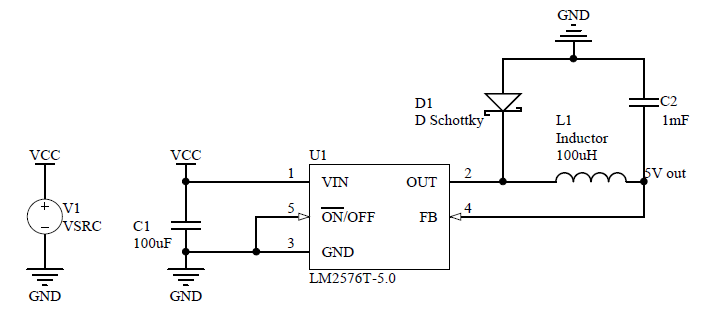
\includegraphics[scale=0.5]{fig/alim_5V.png}
\caption{Figure présentant les plans de l'alimentation 5V pour les périphériques}
\label{fig:alim5V}
\end{figure}

\begin{figure}[htbp]
\centering
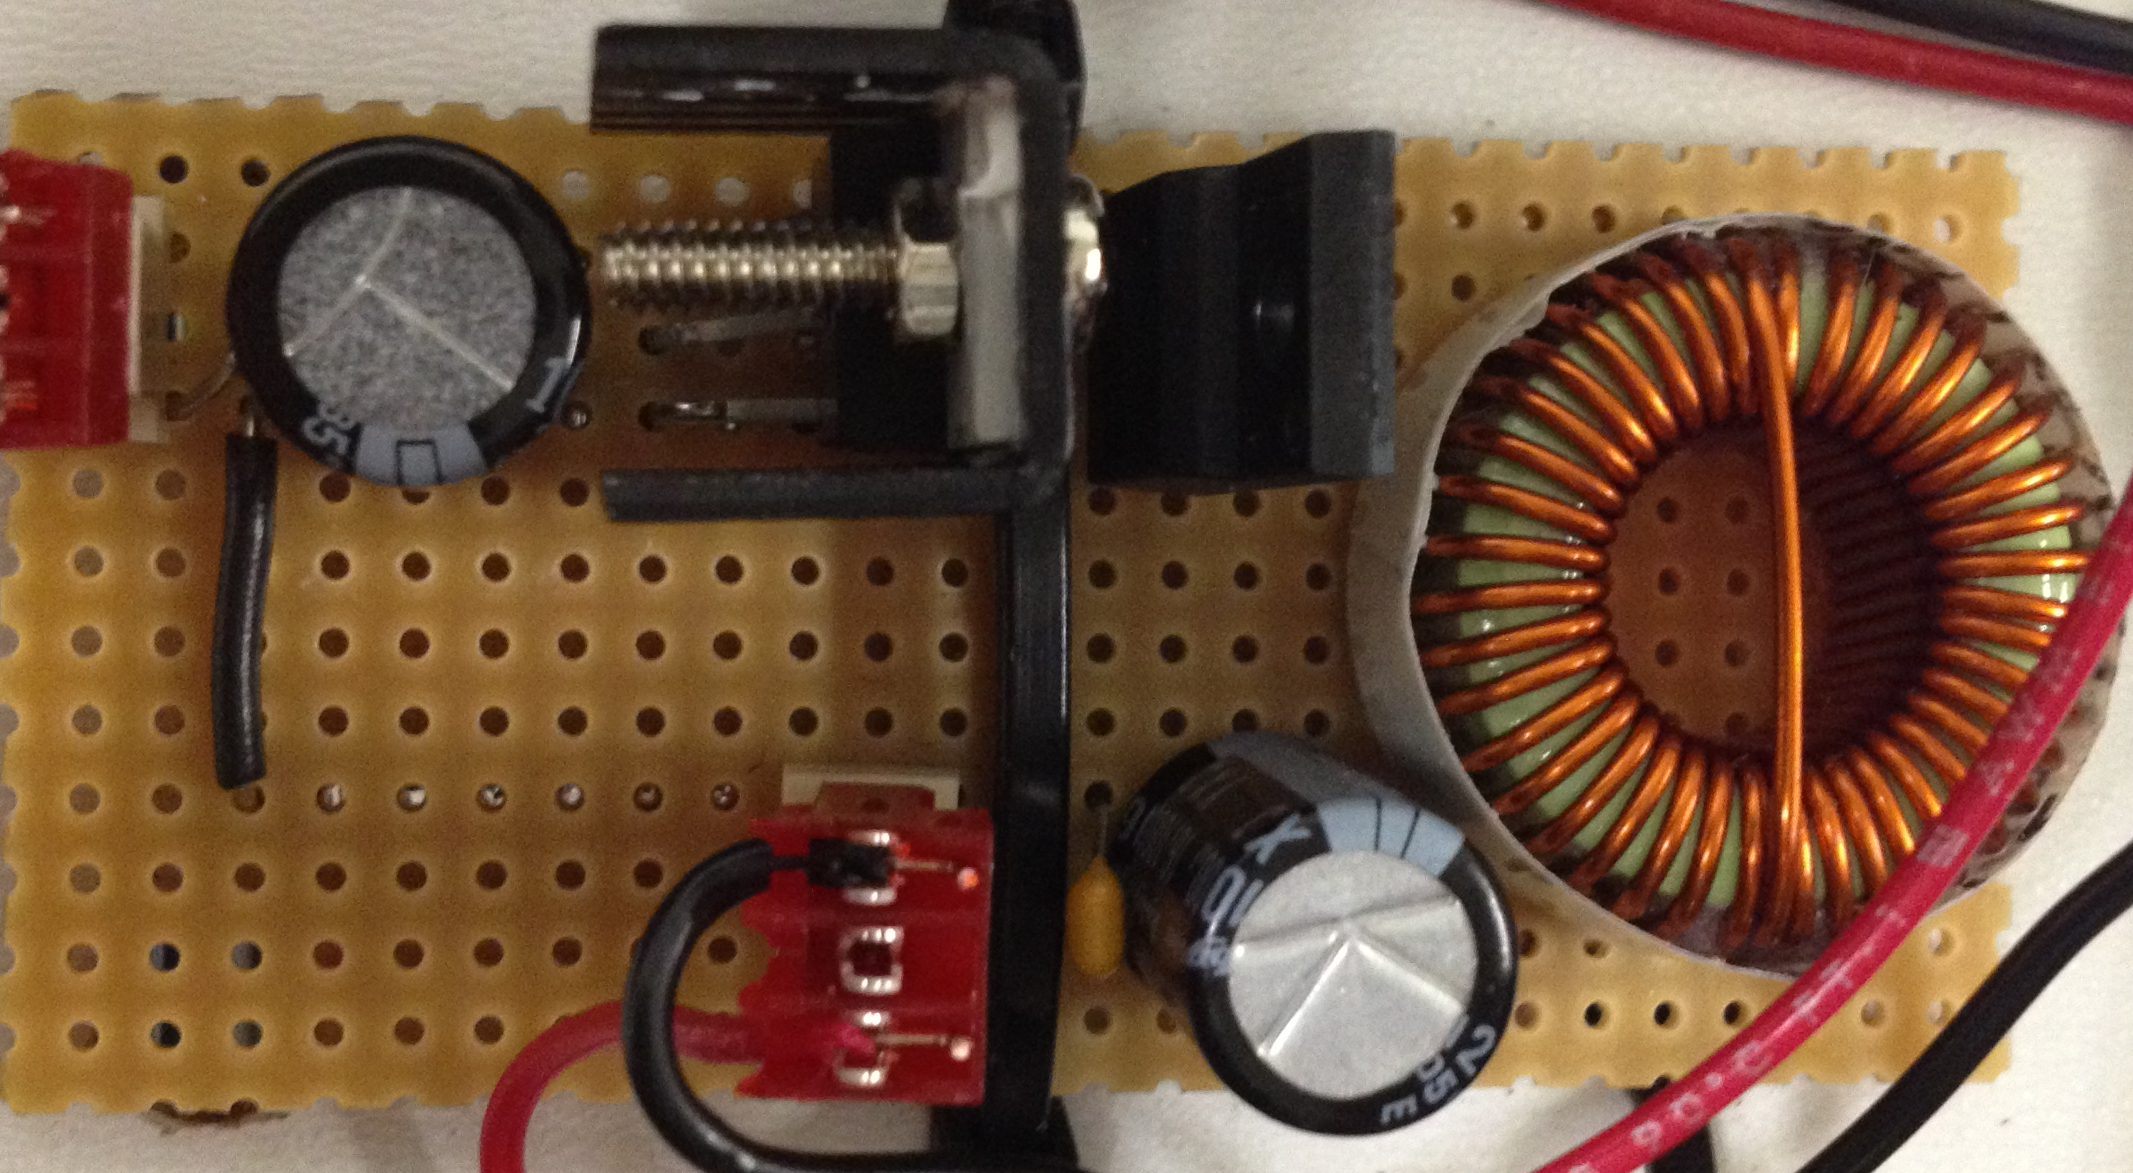
\includegraphics[scale=0.2]{fig/alim_5V_photo.png}
\caption{Figure présentant une photo de l'alimentation 5V pour les périphériques}
\label{fig:alim5Vphoto}
\end{figure}

\section{Alimentation 24V du mac mini et du préhenseur}
L’alimentation 24V, qui alimente le Mac mini ainsi que le préhenseur, a été déjà préconçue et préassemblée sur circuit imprimé, ce qui représentait la solution la plus économique et la plus fiable selon nos hypothèses. Ce module est un hacheur survolteur qui découpe l’alimentation d’entré de 11.1V et la mène à une tension de 24V et cela avec un rendement d’environ 0.94 et de faibles oscillations considérées négligeables. \ref{fig:alim24Vphoto}.

\begin{figure}[htbp]
\centering
\includegraphics[scale=0.1]{fig/alim_24V_photo.png}
\caption{Figure présentant une photo de l'alimentation 24V pour les périphériques}
\label{fig:alim24Vphoto}
\end{figure}

\section{Réception du signal Manchester}
Pour la réception du signal Manchester, nous utilisons un circuit intégré de décodage de tonalité, le LM567, qui met sa patte de sortie à la masse lorsqu’il détecte la fréquence ciblée sur sa patte d’entrée. Nous utilisons un comparateur à hystérésis à la sortie du décodeur pour contourner les variations de tension dues aux variations d’intensités du signal d’entré. Cependant, comme le signal de sortie du décodeur est inversé, nous inversons la sortie du comparateur dans un inverseur pour ensuite envoyer le signal de sortie de celui-ci vers le microcontrôleur qui le traite. Ce récepteur est opérationnel depuis quelques semaines déjà. Le plan de ce récepteur est présenté à la figure 10.5.

\section{Préhenseur}
Le préhenseur est réalisé à l’aide d’un actionneur magnétique qui reçoit une commande de 0V ou 5V qui lui dicte ainsi s’il doit abaisser ou remonter le crayon. Le circuit magnétique exerce une force sur le crayon vers le bas lorsque la commande le lui dicte alors qu’un simple élastique sert de dispositif de retour en place du crayon. Pour minimiser les points morts lors des changements de direction du robot, nous utilisons un système de plongeur qui progresse dans un guide à faible tolérance,  qui maximise ainsi la précision de l’actionneur magnétique qui le précède. Pour actionner le préhenseur, nous utilisons la commande de 0-5V, fournie par le microcontrôleur, sur la gâchette d’un transistor mosfet qui limite la puissance fournie par le microcontrôleur. Le préhenseur et son système de commande sont opérationnels depuis un certain temps déjà. On peut observer le schéma du circuit de l’actionneur sur la figure 10.6.

\section{DEL verte de fin de tâche}
Pour le circuit de la DEL verte qui confirme la fin des tâches du robot, nous utilisons un transistor mosfet de faible puissance qui reçoit la commande du microcontrôleur sur sa gâchette et permet le contrôle de celle-ci. On peut observer le schéma du circuit de commande de la DEL sur la figure 10.7.

\section{Circuit de protection}
Pour le circuit de protection nous avons utilisé trois fusibles en série avec des interrupteurs pour alimenter chacun des circuits d’alimentation 11,1V, 5V et 24V. Chacun des interrupteurs est muni d’un témoin lumineux qui confirme sa mise sous tension et valide que son fusible est intact.

\section{Source d'énergie}
Pour alimenter les différents composants du robot, nous utilisons une batterie lithium Polymère qui est connue pour sa grande capacité énergétique par unité de volume. Nous utilisons donc une pile qui comporte 3 cellules de ce type en série qui produisent une tension totale de 11.1V pour une capacité de 5Ah qui nous permet une autonomie de 30 minutes dans le pire des cas.


\section{Asservissement des moteurs}
\subsection{Modélisation}
L'optimisation des paramètres de réglage a été réalisée grâce à l'utilisation d'un outil de CAO élaboré au moyen de Matlab-Simulink. La fonction de transfert des moteurs a été identifiée au moyen d'une réponse à l'échelon et de l'outil \textit{ident} de Matlab. L'ordre choisi de la fonction est élevé et présente une concordance de 94\% avec la réponse obtenue expérimentalement. L'outil \textit{pidtool} permet par la suite de configurer adéquatement le PIDF et d'obtenir la réponse souhaitée et les paramètres associés. Suivant ces paramètres, le PIDF présent dans le microcontrôleur est ajusté.
\paragraph{}L'usage de l'outil interactif permet d'optimiser la réponse et d'obtenir des paramètres de préréglages qui limitent le nombre d'itérations. La réponse obtenue logiciellement est présentée à la figure \ref{fig:as_1}
\begin{figure}[htbp]
\centering
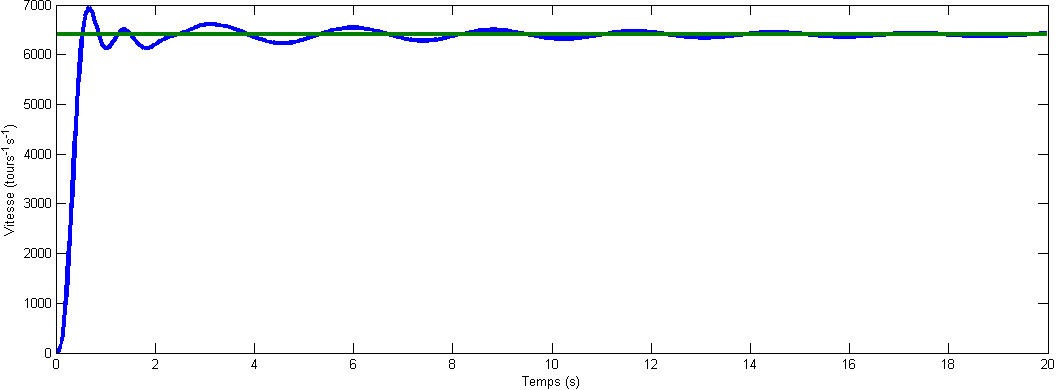
\includegraphics[scale=0.6]{fig/asservissement_1.png}
\caption{Figure présentant la réponse à un échelon de consigne de 6400$\left[tours^{-1}s^{-1}\right]$ du système régulé au moyen du régulateur optimisé dans simulink}
\label{fig:as_1}
\end{figure}
\subsection{Implantation pratique}
\label{s:ass_implantation_pratique}
La réponse à un échelon de consigne de 6400 ($tours^{-1} s^{-1}$) avec les paramètres de réglage réels est présentée à la figure \ref{fig:as_2}. À noter que les consignes en $tours^{-1} s^{-1}$ indique la vitesse en nombre de 1/6400 de tours de roue. Cette fraction de tour est due au fait que les interfaces d'encodeurs en quadratures captent 6400 transitions par tour complet de roue (voir la sous-section \ref{asservissement_mesures} pour plus de détails).
Le système a été implanté avec un asservissement en vitesse et sans asservissement de position. Les expériences pratiques réalisées montrent que l'évolution de la position est linéaire, et ce, sans asservissement. La figure \ref{fig:as_3} présente ce phénomène pour une consigne de 6400 ($tours^{-1} s^{-1}$) qui vise à amener le système à une position de 9100 $tours^{-1}$.
En utilisant les paramètres obtenus dans Matlab comme point de départ, les paramètres de réglages ont été modifiés de manière à obtenir des réponses remplissant les critères de stabilité, de vitesse et de dépassement souhaités. Afin d'améliorer la vitesse des déplacements, différents PID ont été ajustés selon différentes vitesses d'asservissement. On compte 3 de ces PID pour les déplacements unilatéraux et 1 déplacement réservé pour les mouvements reliés au dessin. La différence est que la vitesse de dessin est beaucoup plus basse que celle du déplacement usuel en vue de permettre une plus grande précision. Le moteur n'étant plus très linéaire à ces faibles vitesses (roulement et zone morte très limitants) et le système étant incapable de démarrer de lui même pour procéder à l'identification, le PID a donc été ajusté de manière manuelle, par itérations. Les PID sont fonctionnels et les systèmes stables, cependant, la décélération avant l'arrêt et le positionnement critique se font par l'entremise d'un palier de ralentissement à une vitesse intermédiaire avant freinage. Ces courbes de décélérations sont à mettre au point avant de pouvoir entamer le contrôle en dessin. Par ailleurs, les mouvements en diagonale ne sont pas encore parfaitement au point et requièrent quelques heures de travail additionnelles.
\begin{figure}[htbp]
\centering
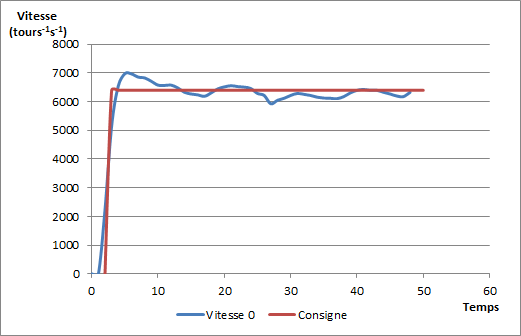
\includegraphics[scale=0.6]{fig/asservissement_3.png}
\caption{Figure présentant la réponse à un échelon de consigne de 6400$\left[tours^{-1}s^{-1}\right]$ du système régulé au moyen du régulateur réel et de la réponse en position associée}
\label{fig:as_2}
\end{figure}
\begin{figure}[htbp]
\centering
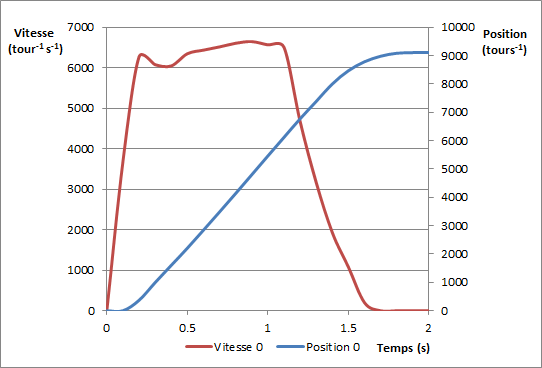
\includegraphics[scale=0.6]{fig/asservissement_2.png}
\caption{Figure présentant la réponse à un échelon de consigne de 6400$\left[tours^{-1}s^{-1}\right]$ du système régulé au moyen du régulateur réel et de la réponse en position associée}
\label{fig:as_3}
\end{figure}
\subsection{Implantation électronique}
\subsubsection{Les prises de mesures}
\label{asservissement_mesures}
Pour prendre des mesures de positions et de vitesses pour effectuer l'asservissement, nous utilisons deux QEI (Quadrature Encoder Interface) matériels qui sont sur le microcontrôleur. Ces deux interfaces prennent en entrée les sorties des encodeurs situés sur les moteurs et captent les transitions lors de la rotation des moteurs. Puisqu'il y a deux senseurs placés en quadrature sur chaque moteur, on peut détecter la direction de la rotation des moteurs. À prendre note qu'un signal transmis par un encodeur contient 64 transitions par tour complet de moteur et que le ratio de la rotation moteur:roue est 100:1. Un signal transmis par un encodeur contient alors 6400 transitions pour une rotation complète de roue. Pour les deux autres moteurs, nous avons réalisé deux interfaces d'encodeurs en quadratures logicielles à l'aide de deux broches d'entrées/sorties par interface, de courtes interruptions et d'une machine à états. Les interruptions sont lancées lorsqu'une transition est détectée sur l'une des broches. L'état des broches est alors lu et sauvegardé pour être traité par la machine à états. La machine à états utilisée est illustrée à la figure \ref{fig:cytron_machine_etats}. Les 0 et 1 indiqué dans les cercles identifient l'état logique des broches. Les -1 ou +1 tracés au dessus des transitions indiquent s'il faut incrémenter ou décrémenter la position de la roue en rotation.
\begin{figure}[htbp]
\centering
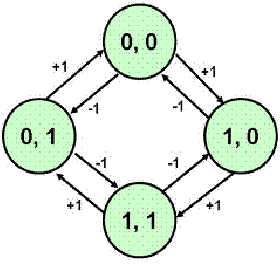
\includegraphics[scale=0.7]{fig/cytron_machine_etats.png}
\caption{Machine à états servant d'interface d'encodeur en quadrature (Cytron. Quadrature Encoder. \url{http://tutorial.cytron.com.my/2012/01/17/quadrature-encoder/}, consulté le 3 mars.)}
\label{fig:cytron_machine_etats}
\end{figure}
\subsubsection{PID}
Le PID utilisé pour l'asservissement est une courte fonction réalisée dans le microcontrôleur. Cette fonction se retrouve dans l'annexe \ref{s:fonction_PID}. À prendre note que l'argument "I" est l'intégrale de l'erreur et "dt" est la différence en temps entre chaque exécution de l'asservissement des moteurs. Cette fonction est exécutée individuellement pour chaque moteur. Des pointeurs transmis en argument indiquent l'emplacement en mémoire des valeurs de chaque moteur utilisées dans le PID. Ensuite, la fréquence d'exécution de la fonction est gardée constante à l'aide d'un timer dans le microcontrôleur qui déclenche une interruption à chaque période et lance l'exécution de l'asservissement.
\subsubsection{Ajustement de la vitesse selon la positon}
Comme indiqué précédemment, pour que le robot atteigne la consigne de position, la vitesse de la rotation des roues doit être ajustée selon la distance restante entre le robot et le point de destination. Cette ajustement est implanté par une simple multiplication d'un certain pourcentage avec la consigne de vitesse lorsque la distance restante à parcourir sera de "X" $tour^{-1}$. Le pourcentage utilisé présentement est hypothétique et sera ajusté lorsque les courbes de décélérations discutées dans la section \ref{s:ass_implantation_pratique} seront identifiées.

\section{Servomoteurs de la Webcam}
Pour contrôler les servomoteurs de la webcam, nous utilisons le contrôleur Micro Maestro de Pololu. Pour le programmer/configurer nous utilisons l'application "Maestro Control Center". Les servomoteurs et le Micro Maestro sont alimentés par l'alimentation 5V. De plus, les servomoteurs reprennent une position prédéterminée lorsque ceux-ci et le Micro Maestro sont alimentés et restent fixes pour permettre à la Webcam de rester immobile même lorsque le robot est en mouvement. Prochainement, un script sera implanté dans le Micro Maestro à l'aide du "Maestro Control Center" pour transmettre par USB une commande du Mac Mini au contrôleur un changement de position des servomoteurs. Cela a pour but de changer l'angle de la Webcam par rapport au sol. Ce changement est nécessaire pour détecter l'orientation du robot.

\section{Extraction des sudocubes}
\subsection{Composantes du système}
L'algorithme pour extraire les sudocubes est séparé en deux : une classe qui traite une photo afin d'extraire les informations d'un sudocube et un lecteur de chiffres. L'extracteur de sudocubes passe des images au lecteur de chiffres afin d'identifier le chiffre présent. 

\begin{figure}[htbp]
\centering
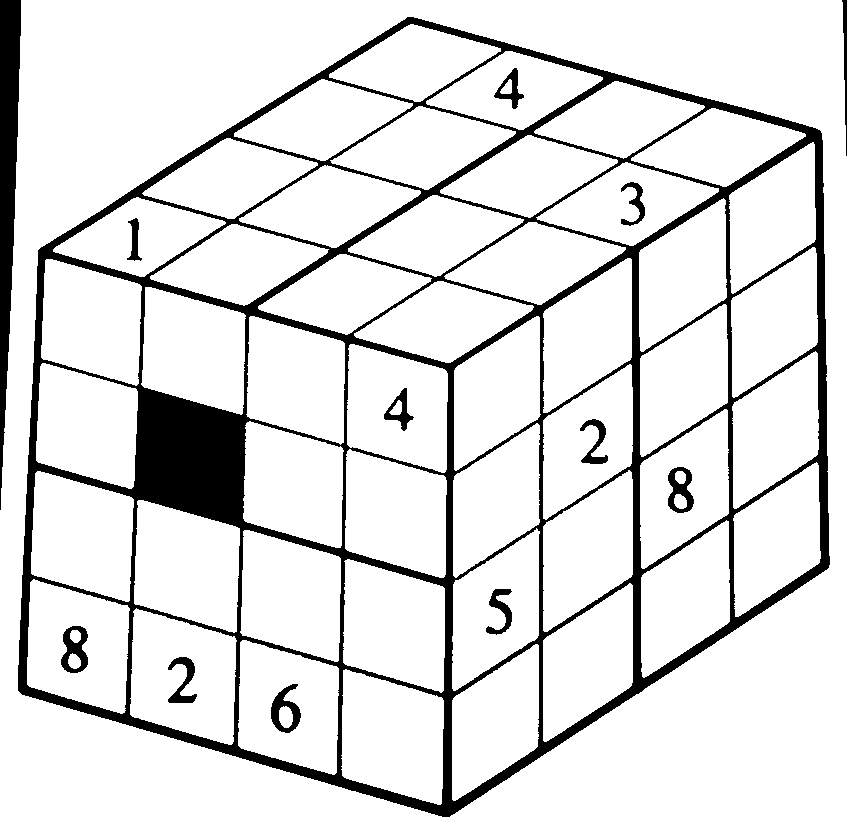
\includegraphics[scale=0.25]{fig/sudocubeThreshold.png}
\caption{Figure présentant un sudocube traité afin d'extraire les informations des cases}
\label{fig:sudoThresh}
\end{figure}

\begin{figure}[htbp]
\centering

\includegraphics[scale=0.9]{fig/chiffresLues.png}
\caption{Figure présentant un exemple d'images extraites des cases du sudocube et normalisées avant d'être passées au lecteur de chiffres}
\label{fig:chifLu}
\end{figure}

\subsection{Les solutions retenus/considérés}
Pour le lecteur de chiffres, deux solutions furent considérées : la librairie Tesseract et l'algorithme d'intelligence artificielle KNearest implanté dans la librairie OpenCV. Tesseract est une librairie qui permet de faire la lecture de caractères de plusieurs langues. Nous avons jugé que cette solution offre des fonctionnalités superflues en plus d'imposer une dépendance supplémentaire au projet. Puisqu’OpenCV est une dépendance obligatoire et que la méthode KNearest nous permet d'obtenir le même résultat qu'avec Tesseract nous avons choisi cette solution.

\subsection{Les moyens utilisé pour configurer}
L'extracteur de sudocube fut configuré (seuils, coefficients de dilatation et d'érosion) à partir d'un lot de tests de 42 images (angles, distances sudocube/robot et luminosités variées). La configuration fut réalisée par essais/erreur pour trouver les paramètres optimaux pour toutes les images.

Le lecteur de chiffres est entraîné avec 40 échantillons par chiffres. Puis, testé avec un lot de 60 nouvelles images par chiffres afin de vérifier sa robustesse.

\section{Solveur de Sudocubes}
<<<<<<< HEAD
=======
\subsection{Composantes du solveur}
L'algorithme qui solutionne les sudocubes a été développé en C++. L'utilisation de la programmation par contraintes (CSP) aurait été  plus simple à implanter et nous aurait fait économiser du temps, mais nous n'avions pas envisagé cette solution au départ. Nous avions déjà un prototype au moment notre prise de conscience de l'existence de ce type de programmation. Le développement du solveur est actuellement terminé et il fonctionne.
>>>>>>> cb9a91c16df60e1f04b7ff48c2271ddbc87a3a82

\subsection{Composantes du solveur}
L'algorithme qui solutionne les sudocubes a été développé en C++. L'utilisation de la programmation par contraintes (CSP) aurait été  plus simple à implanter et nous aurait fait économiser du temps, mais nous n'avions pas envisagé cette solution au départ. Nous avions déjà un prototype au moment notre prise de conscience de l'existence de ce type de programmation. Le développement du solveur est actuellement terminé et il fonctionne.


L'algorithme qui résout les sudocubes a été développé en C++. L'utilisation de la programmation par contraintes (CSP) aurait été  plus simple à implanter et nous aurait fait économiser du temps, mais nous n'avions pas envisagé cette solution au départ. Nous avions déjà un prototype au moment de notre prise de conscience de l'existence de ce type de programmation. Le développement du solveur est actuellement terminé et il fonctionne.
Il utilise une structure de données afin de garder en mémoire le sudocube qui n'est en fait qu'un simple tableau à trois dimensions. Elle devient donc en même temps une interface pour la vision afin de stocker ses données obtenues lors de l'extraction du sudocube.
Les stratégies utilisées pour résoudre le sudocube sont les mêmes qui sont utilisées dans le monde des sudokus normaux, mais adaptées aux sudocubes. Plus spécifiquement, nous avons utilisé les stratégies (ici citées en anglais pour les retrouver plus facilement sur Internet):\newline
\begin{itemize}
\item Naked pairs
\item Hidden pairs/triples
\item Pointing pairs/triples
\item Box and line reduction
\end{itemize}
\paragraph{}Si ces stratégies ne suffisent pas à résoudre le sudocube, nous utilisons la technique de force brute. Nous pensons que c'est une solution acceptable puisque la probabilité d’occurrence de la situation est faible.
L'algorithme peut trouver une solution à des sudocubes ayant uniquement 4 chiffres au départ. Il satisfait donc les exigences du client étant donné que les sudocubes  présentés au laboratoire ont entre 9 et 14 chiffres. Le temps d'exécution varie de quelques milisecondes à quelques dizaines de milisecondes pour les sudocubes testés.

\paragraph{}Si ces stratégies ne suffisent pas à solutionner le sudocube, nous utilisons la technique de force brute. Nous pensons que c'est une solution acceptable puisque il sera plutôt rare que cette situation surviendra.

L'algorithme peut trouver une solution à des sudocubes ayant uniquement 4 chiffres au départ. Il satisfait donc les exigences du client étant donné que les sudokubes "test" présentés au laboratoires ont entre 9 et 14 chiffres. Le temps d'exécution varie de quelques milisecondes à quelques dizaines de milisecondes pour les sudocubes testés.

\subsection{Stratégie de test}
Pour tester entièrement notre classe solveur, il faudrait tester chacune des stratégies utilisées unitairement. Toutefois, si nous avions voulu tester chacune des stratégies, il aurait fallu adopter une architecture différente, puisque ces stratégies sont des méthodes privées de la classe solveur. Trois choix s'offraient alors à nous.

Premièrement, nous aurions pu briser l'encapsulation de la classe solveur, ce qui n'est généralement pas une bonne pratique.

Sinon, nous aurions pu nous créer un nouvel objet duquel hériteraient chacune des stratégies. De cette façon, les stratégies deviendraient des objets et seraient injectées dans la classe solveur à sa construction, préservant l'encapsulation. On aurait donc l'avantage de pouvoir tester chacune des stratégies unitairement, en plus de pouvoir isoler la classe solveur pour la tester (en utilisant des mocks). Cette façon de procéder correspond en fait au patron de conception "strategy". Cette façon de tester est la meilleure des trois côté qualité de code.

Finalement, nous pourrions préserver l'encapsulation en ne testant tout simplement pas chacune des stratégies. Nous testerions uniquement la méthode "solve" en passant au solveur des sudokubes et en observant le résultat, ce qui ressemble plus à un test d'intégration.

Dans notre cas, nous avons préféré utiliser la troisième option. Nous pensons que de tester ainsi couvrira suffisament notre solveur. Selon nous, ce test est un bon compromis entre le respect du bris d'encapsulation et le fait de tester unitairement chacune des stratégies. Nous savons que la meilleure façon de procéder serait la deuxième. Par contre, dans le cadre du projet, nous considérons que le temps qui serait investi dans l'écriture de ces tests est trop grand par rapport au gain que l'on ferait en qualité de code. Nous préférons mettre du temps ailleurs et y revenir au besoin.

\section{Recherche de chemin}
La fonctionnalité recherche de chemin n’en est encore qu’au stade prototype. Cette fonctionnalité n'a pas reçu beaucoup d'attention depuis le livrable 1. On pourrait donc se fier aux données énoncées dans ce livrable pour connaitre l'état de la recherche de chemin: "L'algorithme A* a été choisi, car il est très rapide et facile à implémenter". Nous savons que la solution développée dans le prototype est viable, mais il reste du travail à faire pour que ce soit fonctionnel. Il faudra entre autres ajouter une couche logicielle afin de réduire le nombre de points dans le chemin trouvé et ainsi réduire le nombre de rotations du robot.
<<<<<<< HEAD

=======
>>>>>>> cb9a91c16df60e1f04b7ff48c2271ddbc87a3a82

\section{Communication microcontrôleur - Mac mini}

La communication entre le Mac mini a été réalisée avec un port série UART avec protocole RS-232 à travers le module ICDI du microcontrôleur LM3S9B92. Nous avons choisi ce protocole en raison de sa simplicité et de la facilité du déverminage par rapport au protocole USB plus complexe. Une interface de communication qui passe des commandes sous forme de caractères a été développée du côté microcontrôleur. Un terminal série écrit en Python et utilisant la librairie Pyserial a été développé du côté ordinateur. Ce terminal pour usage diagnostique est compatible avec Linux et Windows et permet de récolter des données utiles sous forme de fichiers CSV pour le développement et les tests d'asservissement et de décodage d'antenne. Le terminal final aura une forme légèrement différente afin de s'interfacer avec ROS.

\section{Décodage du signal Manchester - partie logicielle}

Le décodage logiciel du signal de l'antenne doit transformer les bits en encodage Manchester en bits traditionnels. La méthode choisie doit être robuste aux changements de taux de transmission de bits, car il est spécifié dans la description du projet que ce taux peut varier de plus ou moins 50 bits / seconde. Parmis les algorithmes permettant de détecter des signaux de taux de transmission inconnu, il en existe deux types principaux : 

\begin{enumerate}
\item{Les algorithmes basés sur l'échantillonnage}

On effectue une mesure du signal à un intervalle prédéfini plus petit que la période du signal mesuré. C'est le décompte des bits consécutifs à zéro et à un qui permet de décoder le signal.

\item{Les algorithmes basés sur les timings} 

On effectue une mesure du temps entre les transitions du signal de zéro à un et de un à zéro. C'est le temps entre les montées et descentes qui permet de décoder le signal.
\end{enumerate}

Puisque le LM3S9B92 possède des compteurs d'usage général qui implémentent une fonction de capture d'événement, nous avons choisi d'utiliser la méthode par timings. Pour l'instant, nous pouvons mesurer des temps entre transitions sur un signal interne au microcontrôleur généré par un PWM.


\section{Orientation du robot}

Pour la détermination d’angle et l’orientation du robot, le choix de la caméra embarquée  est très recommandé pour sa précision comparé à la kinect. \\
Dans un premier temps, nous devons calibrer la caméra. Pour ce faire, deux méthodes s’offrent à nous : l’application de l’algorithme de Zhang ou la calibration avec Opencv. Dans ce cas nous retenons la première méthode, car malgré sa complexité, elle est plus efficace. \\
Ensuite, nous procédons à la détermination d’angle du robot par rapport à la ligne rouge déjà tracée sur la table.  Cette partie est réalisée grâce à un traitement d’image supportant la variation de luminosité, d’ombres… ainsi que grâce à des règles de trigonométrie.\\
Enfin,  la détermination de l’orientation du robot (N, S, E, O) est effectuée par la détection des coins de la table. 
L’algorithme de cette opération est assez simple. Si la caméra détecte le coin orange avant le bleu, le robot sera orienté vers le Nord. Si elle détecte le coin bleu avant le coin orange, le robot sera orienté au Sud. La détection des deux coins bleus montrera une orientation vers l’Ouest et enfin la détection des deux coins orange montrera une orientation vers l’Est.\\
Les deux dernières parties sont commencées mais ne sont pas encore complétées à ce jour.


\section{Vision par Kinect}
Pour aider au déplacement du robot, la Kinect à été utilisée pour détecter la position des obstacles, la position du robot lui-même ainsi que sa position angulaire par rapport au point (0.0) de notre représentation cartésienne de la table. Toutefois, comme la Kinect est située à l'extérieur de la table de jeu, il a fallu effectuer une translation et une rotation des données obtenues pour positionner avec exactitude les objets. Les 3 sections qui suivent expliquent en détail les différentes parties de l'algorithme de vision de la Kinect.

\subsection{Transformation des distances}
En premier lieu, il est important de clarifier quelles distances il est possible d'obtenir à l'aide de la Kinect. Le «Framework» OpenNI est capable de retourner 2 types de distances pour chacun des points dans l'image infrarouge obtenue de la Kinect. Le premier type de distances retourné est la longueur en mètre entre l'objectif et un point quelquonque sur l'image. Le second type est dérivé du premier et correspond aux composantes X, Y et Z du vecteur de longueur entre l'objectif et la cible. Pour aider à la compréhension, les deux types de distances peuvent être représenté par les ligne verte sur l'image \ref{fig:kinect_distance}. Toutefois, comme l'origine de notre représentation cartésienne de la table est situé sur le coin inférieur droit de la table et que la Kinect n'est pas situé à cet endroit, il est nécessaire d'obtenir la distance X et Y (lignes bleues sur l'image \ref{fig:kinect_distance}) entre l'origine et le point ciblé sur l'image obtenue de la Kinect. Pour y arriver, il suffit d'obtenir la position X et Y (lignes rouges sur l'image \ref{fig:kinect_distance}) de la lentille infrarouge de la Kinect ainsi que l'angle de la Kinect avec l'axe X de la table. Avec ces valeurs, dans notre cas 14cm, -56cm et $23.5^o$, nous avons mis en oeuvre un logiciel qui permet la transformation des distances de la Kinect vers les composantes X et Y recherchée à l'aide de règles de trigonométrie simples. Cet algorithme permet d'obtenir avec une précision de plus ou moins 1cm pour n'importe quel point situé sur l'image obtenue avec la Kinect. 

\begin{figure}[htbp]
\centering
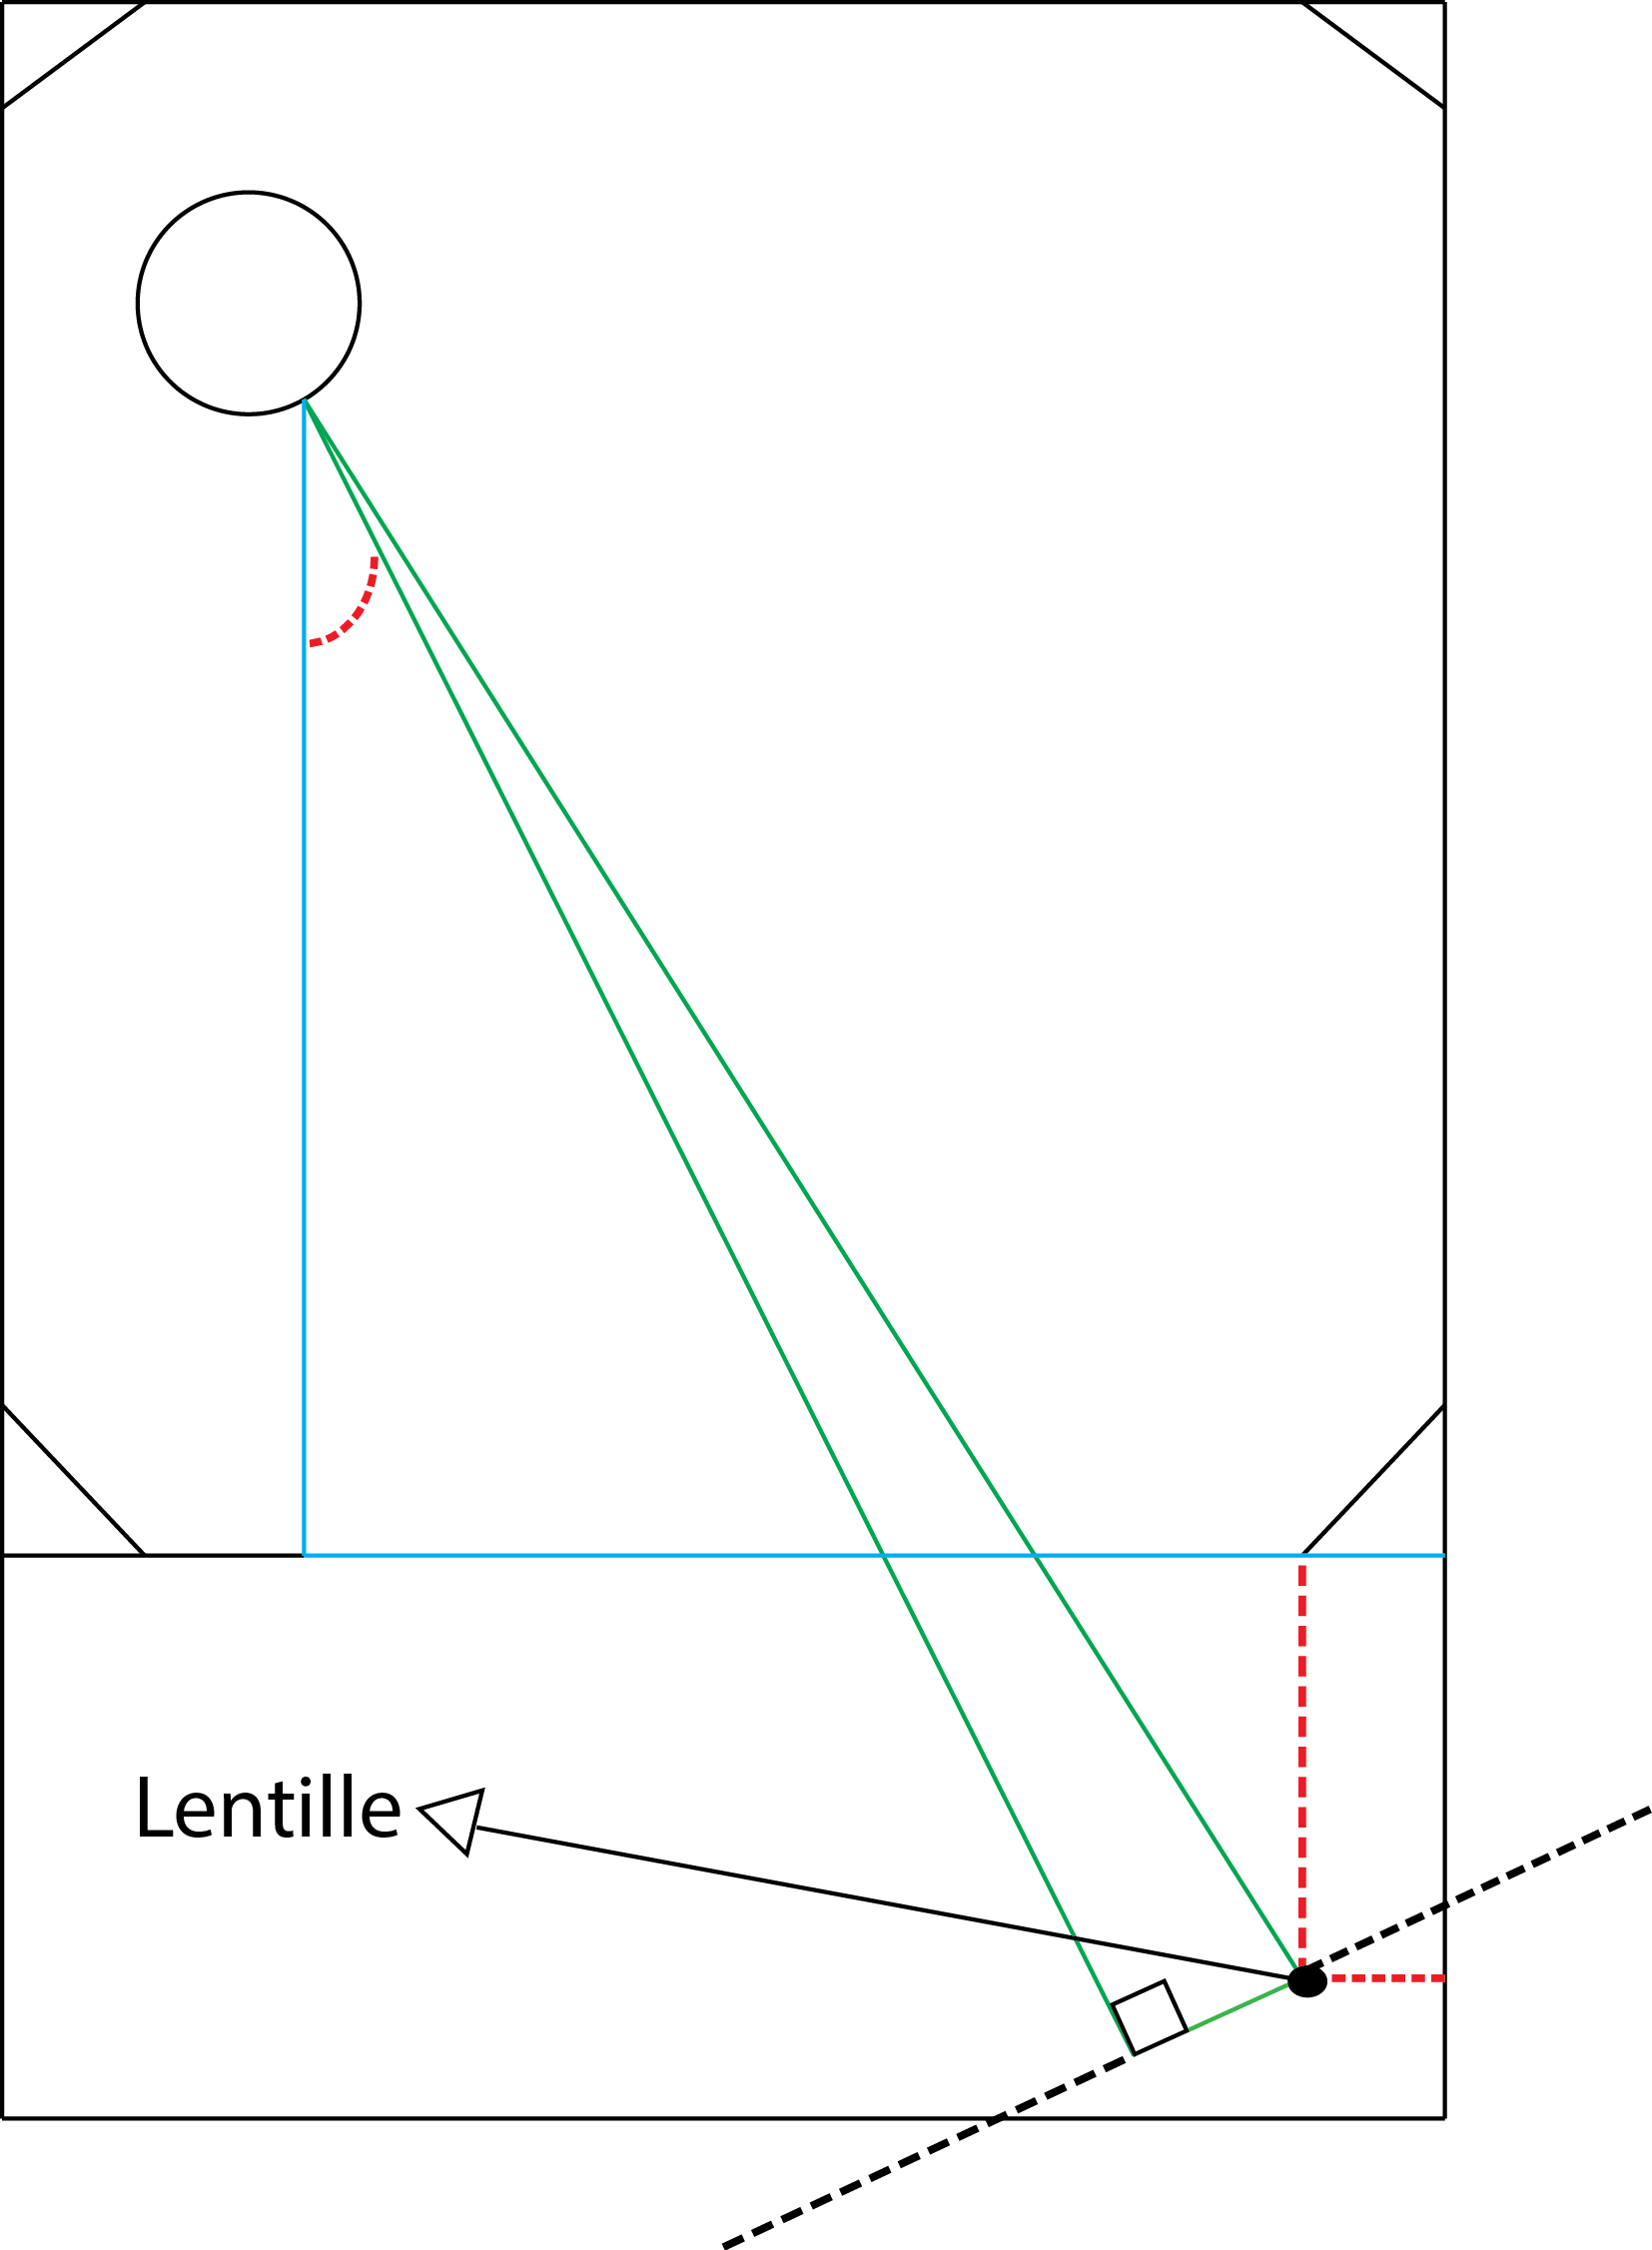
\includegraphics[scale=0.5]{fig/kinect_distance.png}
\caption{Schéma représentant la table et les différentes mesures obtenues avec la Kinect pour un point quelquonque}
\label{fig:kinect_distance}
\end{figure}

\subsection{Détection des obstacles}
Maintenant que nous pouvons obtenir n'importe quelle distance entre l'origine et un point quelquonque sur l'image, nous avons créé l'algorithme de recherche d'obstacles. Sachant que les obstacles sont situés dans une zone précise sur la table et que ceux-ci font 40cm de hauteur, il suffit de rechercher tout objet de cette hauteur et situé dans la zone prédefinie. Comme la Kinect est capable de retourner la hauteur de chacun des points sur l'image infrarouge, il a été facile de trouver les obstacles de cette manière. De plus, à l'aide de simples calculs de statistiques, notre algorithme est capable de trouver les obstacles lorsqu'ils sont presque enlignés ou bien les obstacles avec une obstruction comme le robot devant eux. Comme cet algorithme dépend entièrement de l'algorithme précédent, les positions obtenues pour chacun des obstacles possèdent la même incertitude de 1 cm sur chaque mesure de distance effectuée. En ce qui concerne l'efficacité de l'algorithme, différents tests montrent un temps de calcul d'environ 30 ms sur un Core 2 Duo 2.4 GHz pour obtenir la position du centre des deux obstacles.

\subsection{Détection du robot}
En ce qui concerne la détection du robot, un algorithme semblable à la détection des obstacles à été utilisé. Comme le robot possède une hauteur d'environ 20cm et une profondeur semblable, il est possible d'isoler, dans la matrice de distance, un carré qui correspond aux dimensions du robot. De plus, pour améliorer la précision de la détection du robot, nous allons mettre en place une recherche de symboles de couleur spécifique sur le robot à l'aide de la caméra RGB de la Kinect. Avec cette méthode, qui n'est pas encore implémentée, nous devrions être capable d'obtenir la position réelle du robot peut importe sa position sur la table et ce avec une vitesse qui se rapproche de l'algorithme de détection des obstacles. Pour le moment, en se servant seulement de la détection par contrainte de distance, nous sommes capable de détecter le robot avec une incertitude de 5 cm en environ 30 ms si le robot n'est pas situé en arrière d'un obstacle.

\section{Communication entre le Mac mini et la station de base}
\subsection{Composantes du système}
Avant de pouvoir communiquer avec le robot, nous récupérons l’adresse IP du robot grâce à un script bash exécuté lors du démarrage de celui-ci. Le script récupère l’adresse IP et l’envoie sur le site pastebin.com.

Ensuite, nous utilisons ROS pour gérer la communication entre les différents nodes ROS. Une node c’est une application qui utilise l’API de ROS. Actuellement, nous avons testé l’envoi de messages au Mac mini pour démarrer la séquence du robot.

On peut voir sur le diagramme \ref{fig:commNodes} la répartition des nodes sur les différents appareils ainsi que les appareils avec lesquels chaque node travaillent. Nous avons choisi de séparer le node du mac mini en deux afin de simplifier les tests pour les composantes qui communiquent avec le microcontrôleur. Grâce au système de communication de ROS on peut envoyer par ligne de commande des messages afin de déplacer le robot ou encore afficher un message sur l’écran LCD, et ce, sans passer par l’écriture d’une application de tests.

\begin{figure}[htbp]
\centering
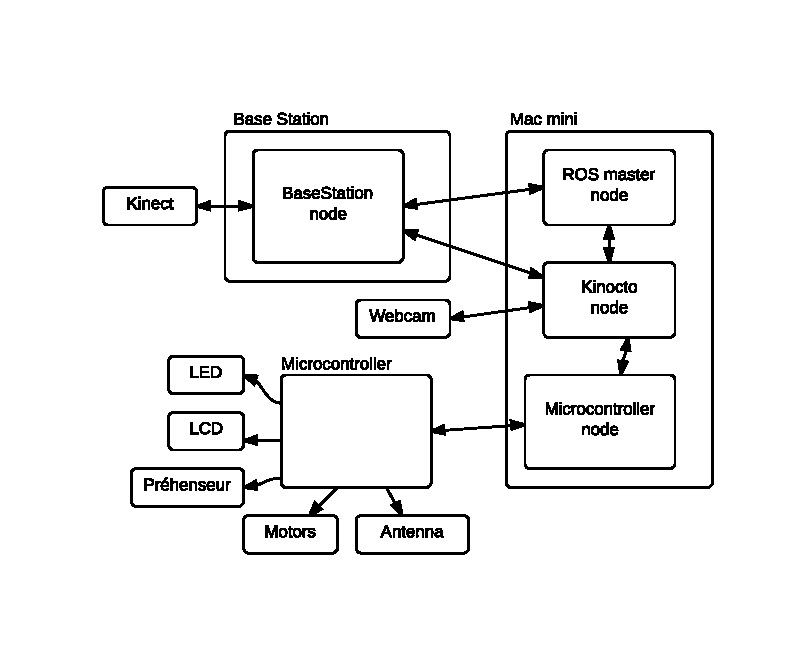
\includegraphics[scale=1]{fig/communicationNodesAppareils.pdf}
\caption{Diagramme représentant la communication entre les nodes et les différents appareils}
\label{fig:commNodes}
\end{figure}

\subsection{Les solutions retenues et considérées}
Nous avons considéré deux solutions : POCO une librairie C++ et ROS un environnement de développement pour robot.

POCO permet d’envoyer des chaines de caractères par TCP/IP. L’envoie de commandes avec POCO consiste en ces étapes : concaténer le nom d’une commande (choisit au préalable) et ses arguments dans une chaine de caractères. Puis, envoyer, à l’aide de la librairie la chaine de caractères. Il faut extraire la commande et ses paramètres lors de la réception d’un message.

ROS fait exactement la même chose que POCO en arrière-plan, mais il y a une couche logiciel qui nous donne des avantages supplémentaires. Pour envoyer des messages, entre deux applications ROS iI suffit de déclarer, pour chaque type de message, des variables et leur type dans un fichier texte. Puis, lors de la compilation du projet ROS génère des struct en C pour chaque message. Ensuite, on utilise l’api de ROS pour définir le contenu des messages et envoyer les messages.

La courbe d’apprentissage est nettement plus prononcée avec ROS. Cependant, avec celui-ci les messages sont hachés avec une somme MD5 et lorsqu’un message est reçu par une node (une application ROS) le contenu est vérifié avec la somme MD5. Nous garantissant ainsi que le message s’est transmis.

De plus, il est possible d’enregistrer tous les messages qui sont envoyés par ROS depuis le démarrage de la séquence, de les consulter séquentiellement dans le temps grâce à une interface graphique et de les exécuter à nouveau afin de reproduire la même séquence de message. C’est un outil de déverminage qui sera utile lors du développement de l’agent intelligent et que l’on ne possède pas avec POCO.

ROS a été retenu pour ses nombreux avantages. 


\appendix
%!TEX root = ../rapport.tex
%!TEX encoding = UTF-8 Unicode
% Chapitres "Annexes"

% modifié par Francis Valois, Université Laval
% 31/01/2011 - version 1.0 - Création du document
\chapter{Annexes}
\label{s:annexes}

\section{Asservissement des moteurs}
\subsection{Fonction agissant comme PID} \label{s:fonction_PID}
\begin{lstlisting}[language=C]
long PIDHandler(volatile long *consigne, volatile long *measured_value, volatile float *I, volatile long *previous_error, float dt)
{
  long error = *consigne - *measured_value;
  *I = *I + error*dt;
  float D = (error - *previous_error)/dt;
  long output = Kp*error + Ki*(*I) + Kd*D;
  *previous_error = error;
  return output;
}
\end{lstlisting}



\end{document}
% Fin du document

